\documentclass[11pt,a4paper]{article}
\usepackage[T1]{fontenc}
\usepackage[utf8]{inputenc}
\usepackage{lmodern}
\usepackage{geometry}
\usepackage{amsmath,amssymb}
\usepackage{booktabs}
\usepackage{graphicx}
\usepackage{float}
\usepackage{hyperref}
\usepackage{xcolor}
\geometry{margin=1in}
\graphicspath{{figures/}}
\setlength{\parskip}{0.6em}
\setlength{\parindent}{0pt}

\title{Mathematical Notes on the Irish Rail Dataset}
\author{Generated from irish-rail-nabber}
\date{2026-05-22 15:57}

\begin{document}
\maketitle

\begin{abstract}
This report uses the current Irish Rail archive as a mathematical object rather than just a live dashboard feed. The production database contains 77,943,752 raw time-series rows from 2026-03-12 23:28:29.988475 to 2026-05-22 14:56:28.625464. For the operational plots, repeated polling rows are collapsed to one latest observation per train-stop over the last 14 days, leaving 146,537 cleaned observations. The main result is simple: most trains are close to time, but the delay distribution has a heavy tail, and the Galway--Oranmore--Athenry corridor remains the clearest high-delay pattern.
\end{abstract}

\section{Data and Cleaning}

The raw database is large because it stores polling snapshots: station boards, live positions, HACON snapshots, train movements, and fetch history. Directly plotting raw rows would mostly measure polling frequency. I therefore deduplicate station-board observations by
\[
(\text{train}, \text{date}, \text{station}, \text{origin}, \text{destination}, \text{scheduled times})
\]
and keep the latest row for each train-stop.

I also apply a robust operational window:
\[
 -30 \leq \text{late minutes} \leq 180.
\]
This keeps 146,537 observations and removes obvious stale cross-day artefacts such as roughly 24-hour late values. This is not hiding disruption; it is separating timetable/data glitches from interpretable delay measurements.

\begin{table}[H]
\centering
\begin{tabular}{lr}
\toprule
Metric & Value \\
\midrule
Cleaned train-stop observations & 146,537 \\
Distinct train/date pairs & 10,901 \\
Stations observed & 161 \\
Route pairs observed & 146 \\
Average delay & 1.83 min \\
Median delay & 0 min \\
P90 delay & 5 min \\
P95 delay & 8 min \\
Within 5 minutes & 90.39\% \\
Over 15 minutes & 1.28\% \\
\bottomrule
\end{tabular}
\caption{Cleaned operational sample for the last 14 days.}
\end{table}

\begin{figure}[H]
\centering
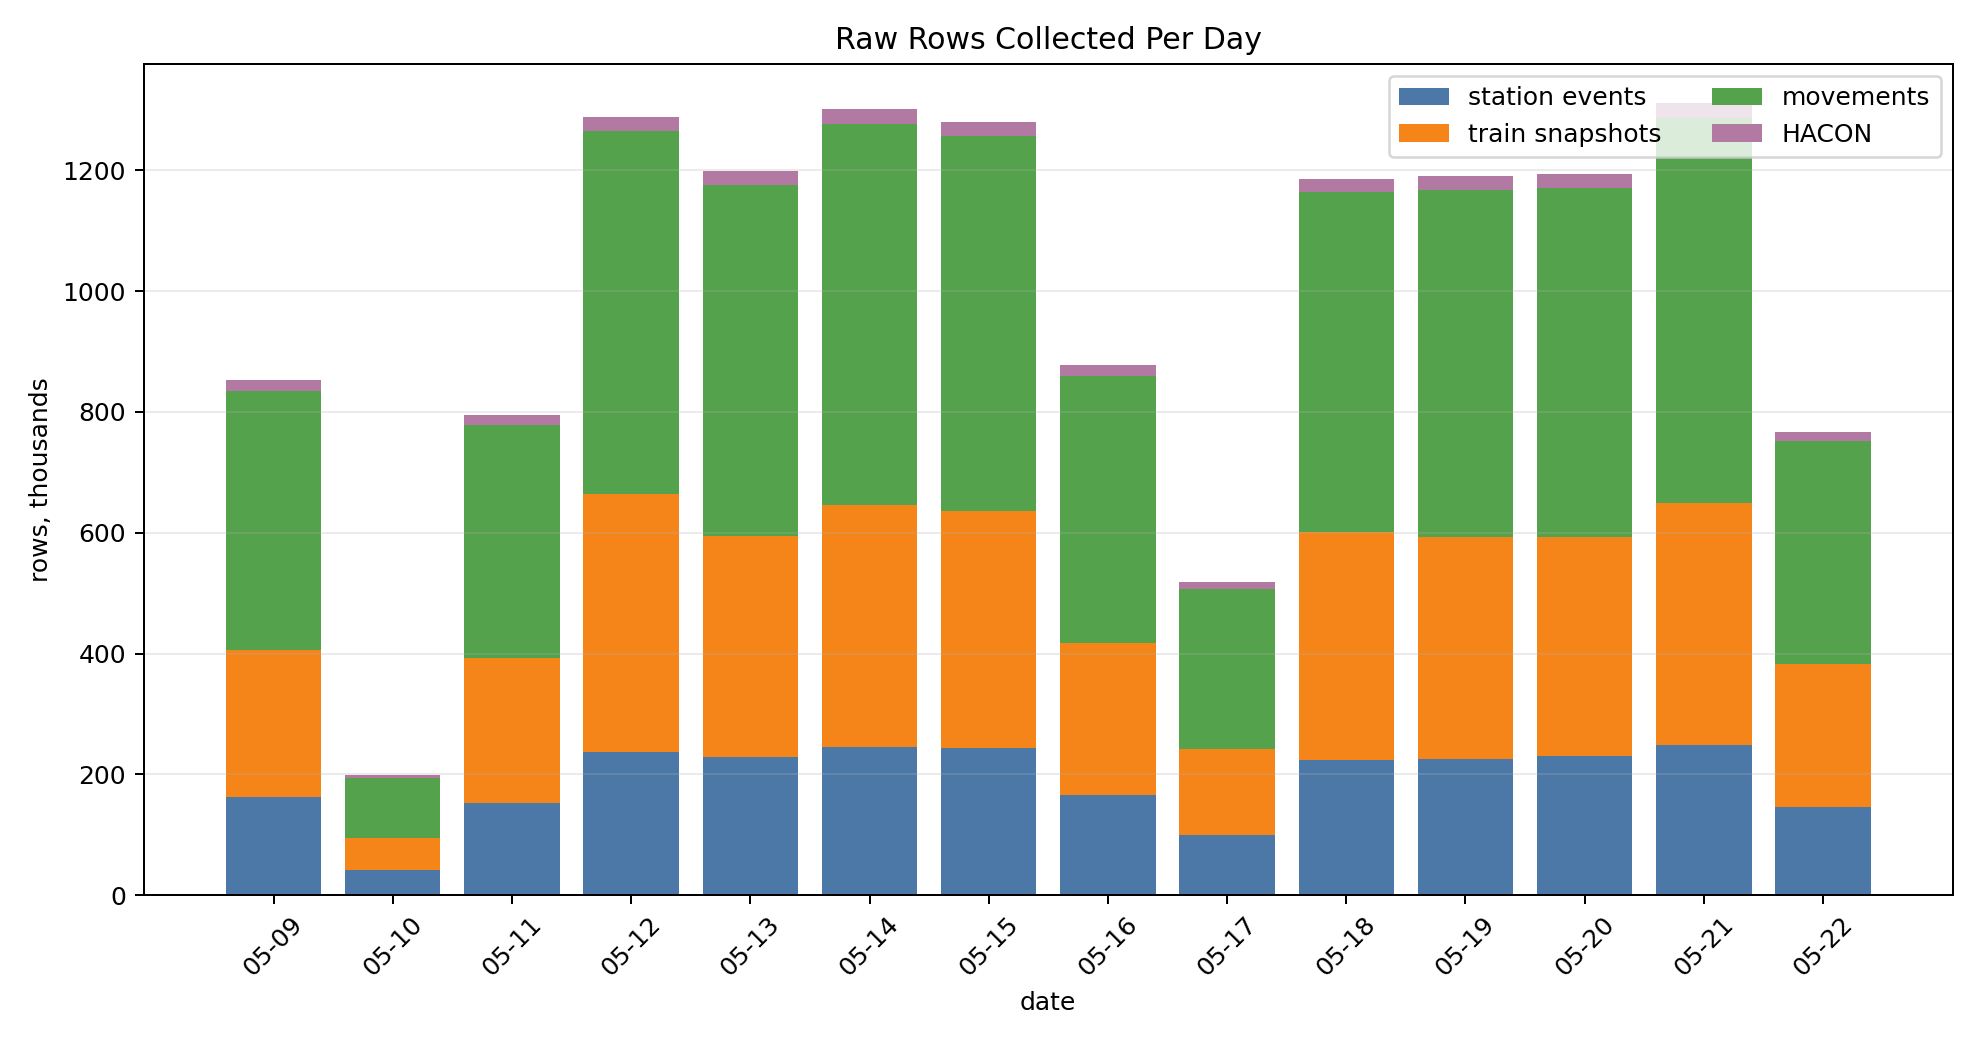
\includegraphics[width=\textwidth]{fig_daily_volume.png}
\caption{Raw rows collected each day. This figure is a pipeline-health view: it shows the scale of the archive, not passenger-facing punctuality.}
\end{figure}

\section{Delay Distribution}

The median delay is 0 minutes, P90 is 5 minutes, and P95 is 8 minutes. This is a heavy-tailed distribution: the ordinary day is good, but the right tail is operationally important.

\begin{figure}[H]
\centering
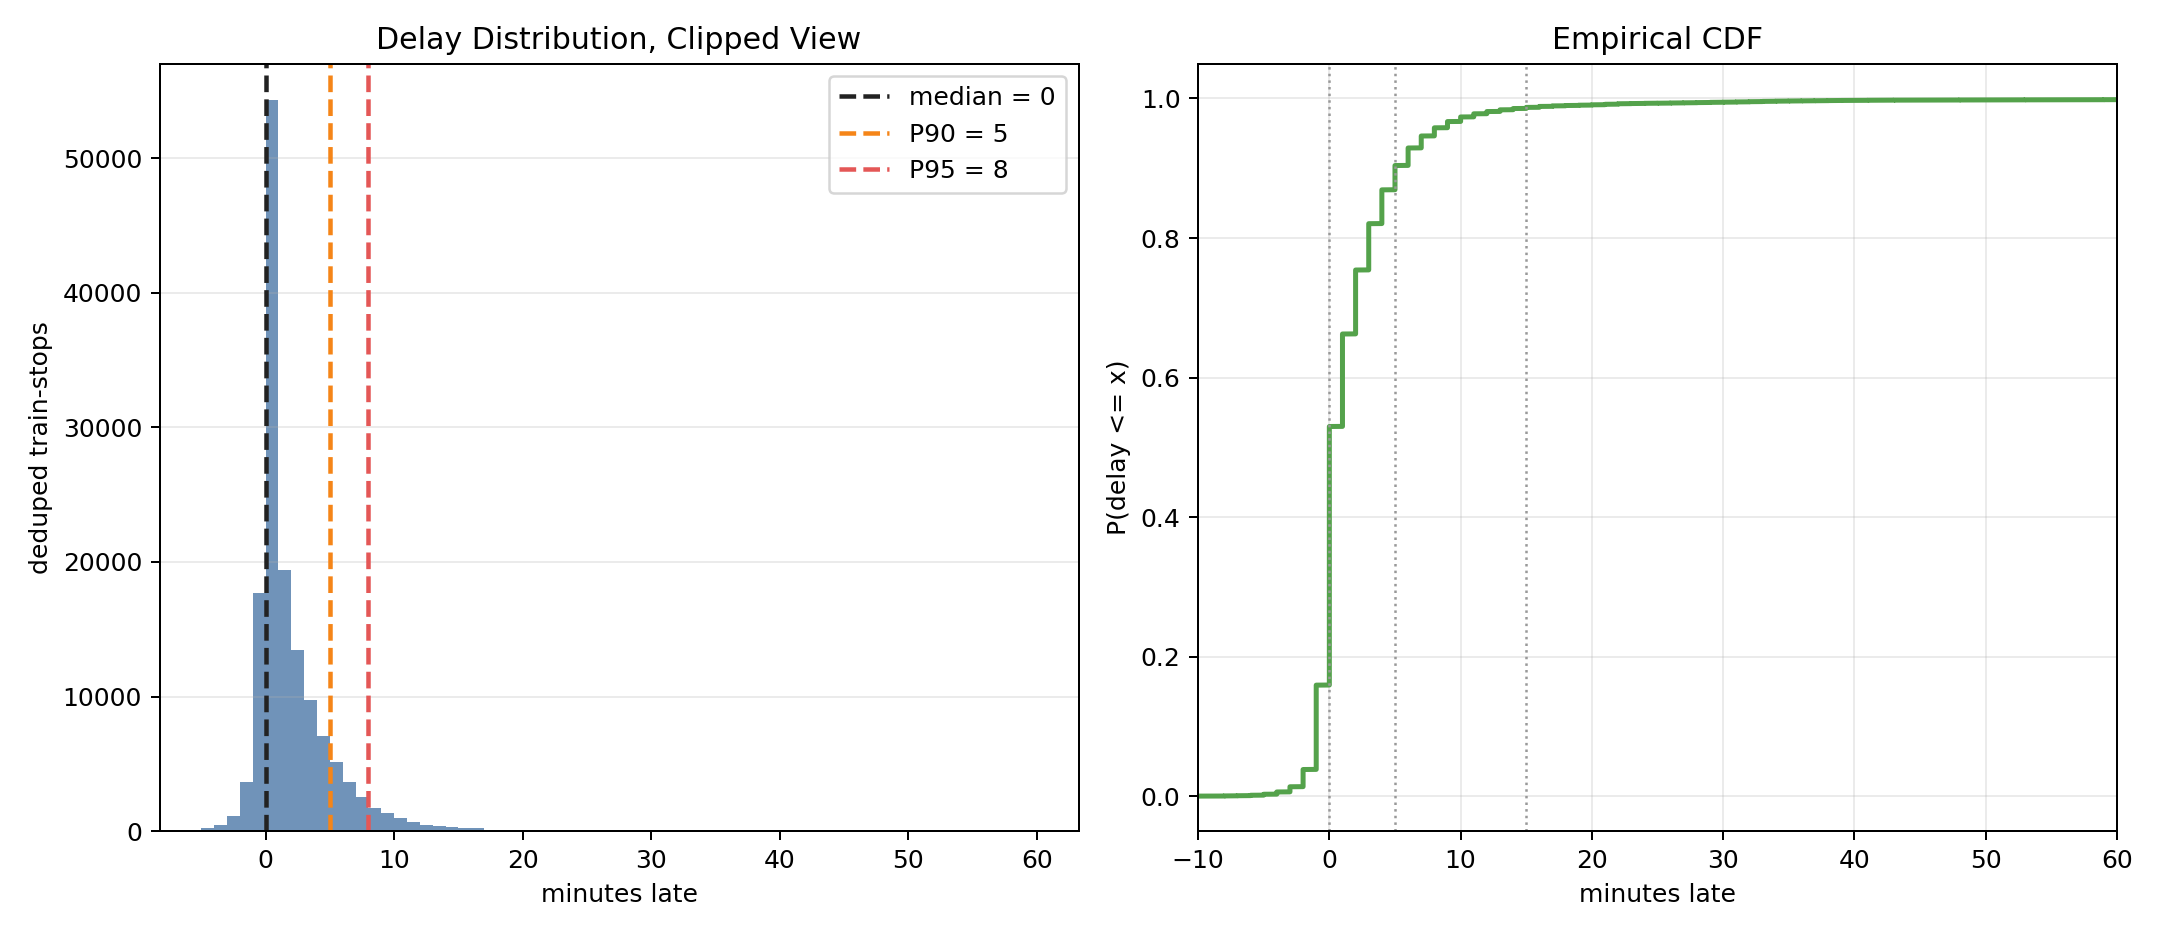
\includegraphics[width=\textwidth]{fig_delay_distribution.png}
\caption{Left: histogram of delay minutes in a readable clipped range. Right: empirical cumulative distribution. The CDF makes the reliability claim clearer than an average: about 90.4\% of cleaned train-stops are within 5 minutes.}
\end{figure}

\section{Time of Day}

The useful statistic here is not just the mean. The P95 line shows when the bad tail grows, while the bars show how much evidence exists in that hour.

\begin{figure}[H]
\centering
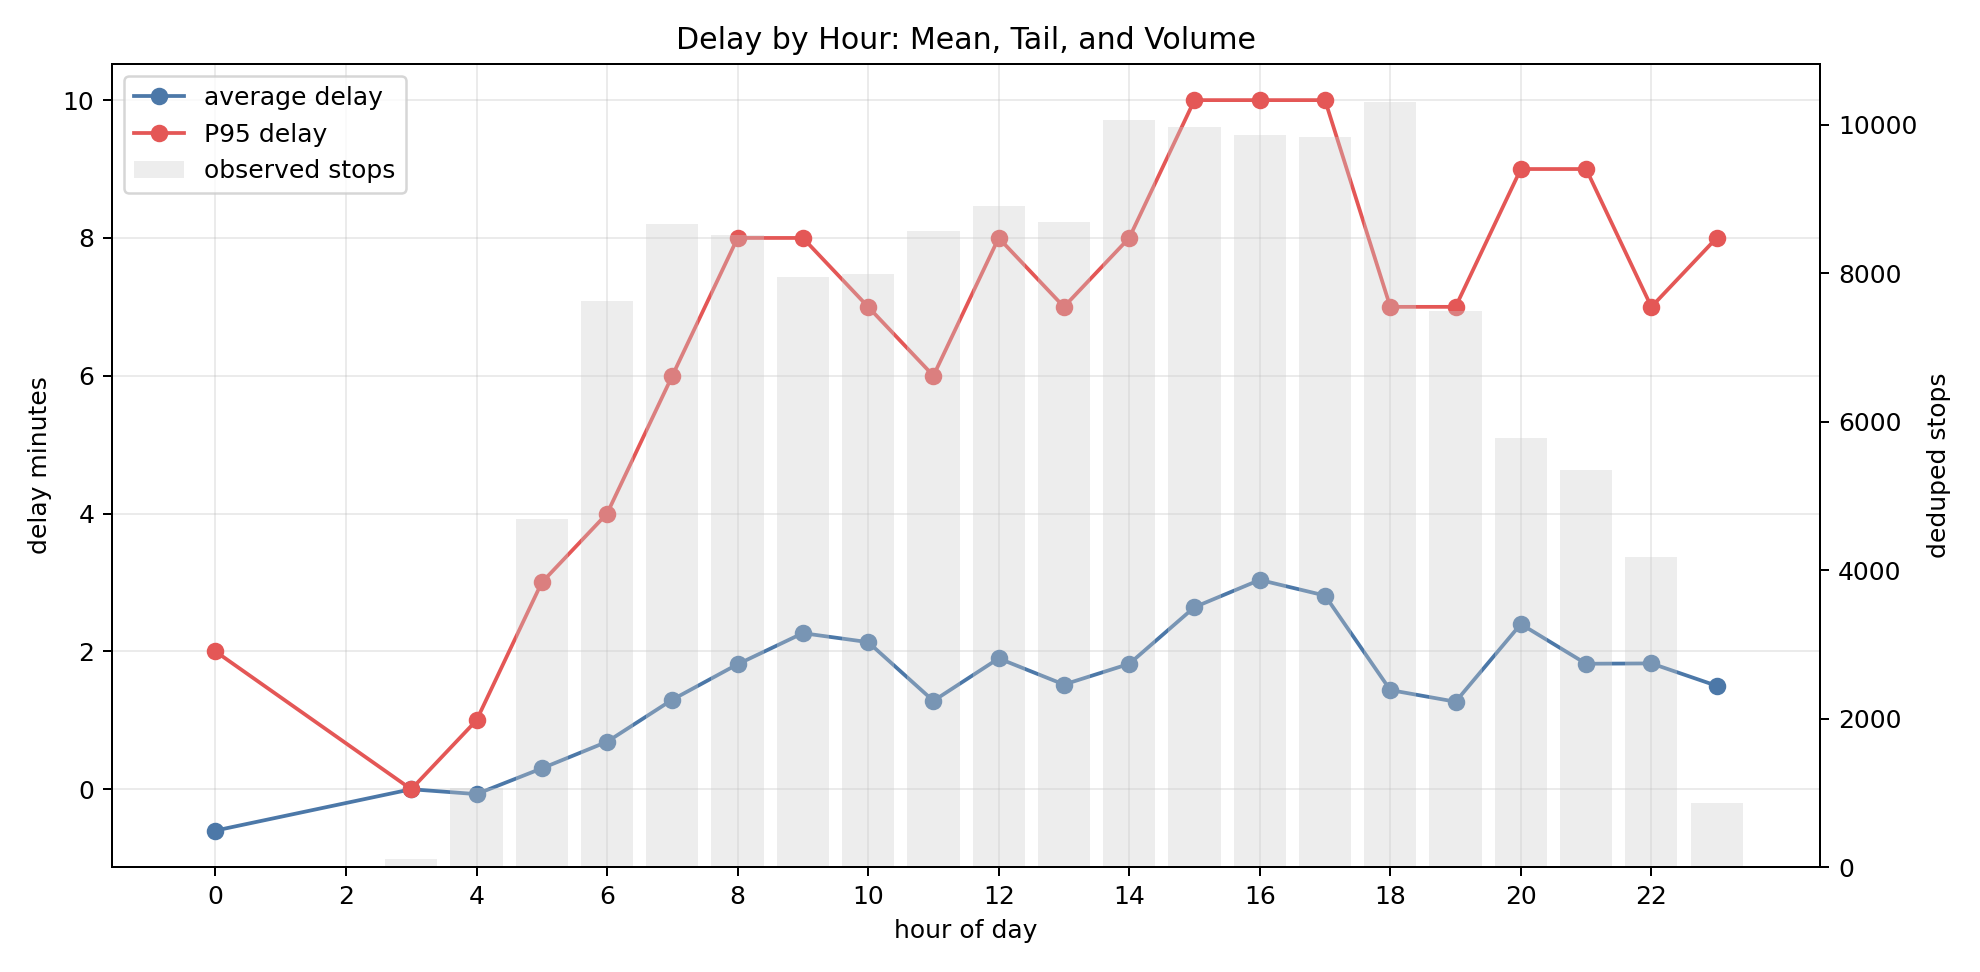
\includegraphics[width=\textwidth]{fig_hourly_delay.png}
\caption{Average delay, P95 delay, and observation volume by hour. Peaks in the P95 curve identify hours where ordinary averages understate passenger risk.}
\end{figure}

\section{Stations and Routes}

\begin{table}[H]
\centering
\small
\begin{tabular}{lrrrr}
\toprule
station & stops & avg & p95 & within5 \\
\midrule
Galway & 502 & 17.25 & 120.00 & 77.09 \\
Oranmore & 461 & 16.61 & 121.00 & 81.13 \\
Athenry & 499 & 15.37 & 102.00 & 78.36 \\
Kilcock & 260 & 5.29 & 16.00 & 66.92 \\
Athy & 262 & 4.69 & 10.00 & 68.70 \\
Enfield & 251 & 3.98 & 16.00 & 76.10 \\
Mullingar & 262 & 3.92 & 16.00 & 77.10 \\
Thurles & 476 & 2.89 & 10.00 & 84.66 \\
Tullamore & 411 & 2.76 & 11.00 & 85.40 \\
Maynooth & 1199 & 2.64 & 10.00 & 84.57 \\
\bottomrule
\end{tabular}
\caption{Highest average-delay stations with at least 250 cleaned observations. Values are in minutes except within5, which is percent.}
\end{table}

\begin{figure}[H]
\centering
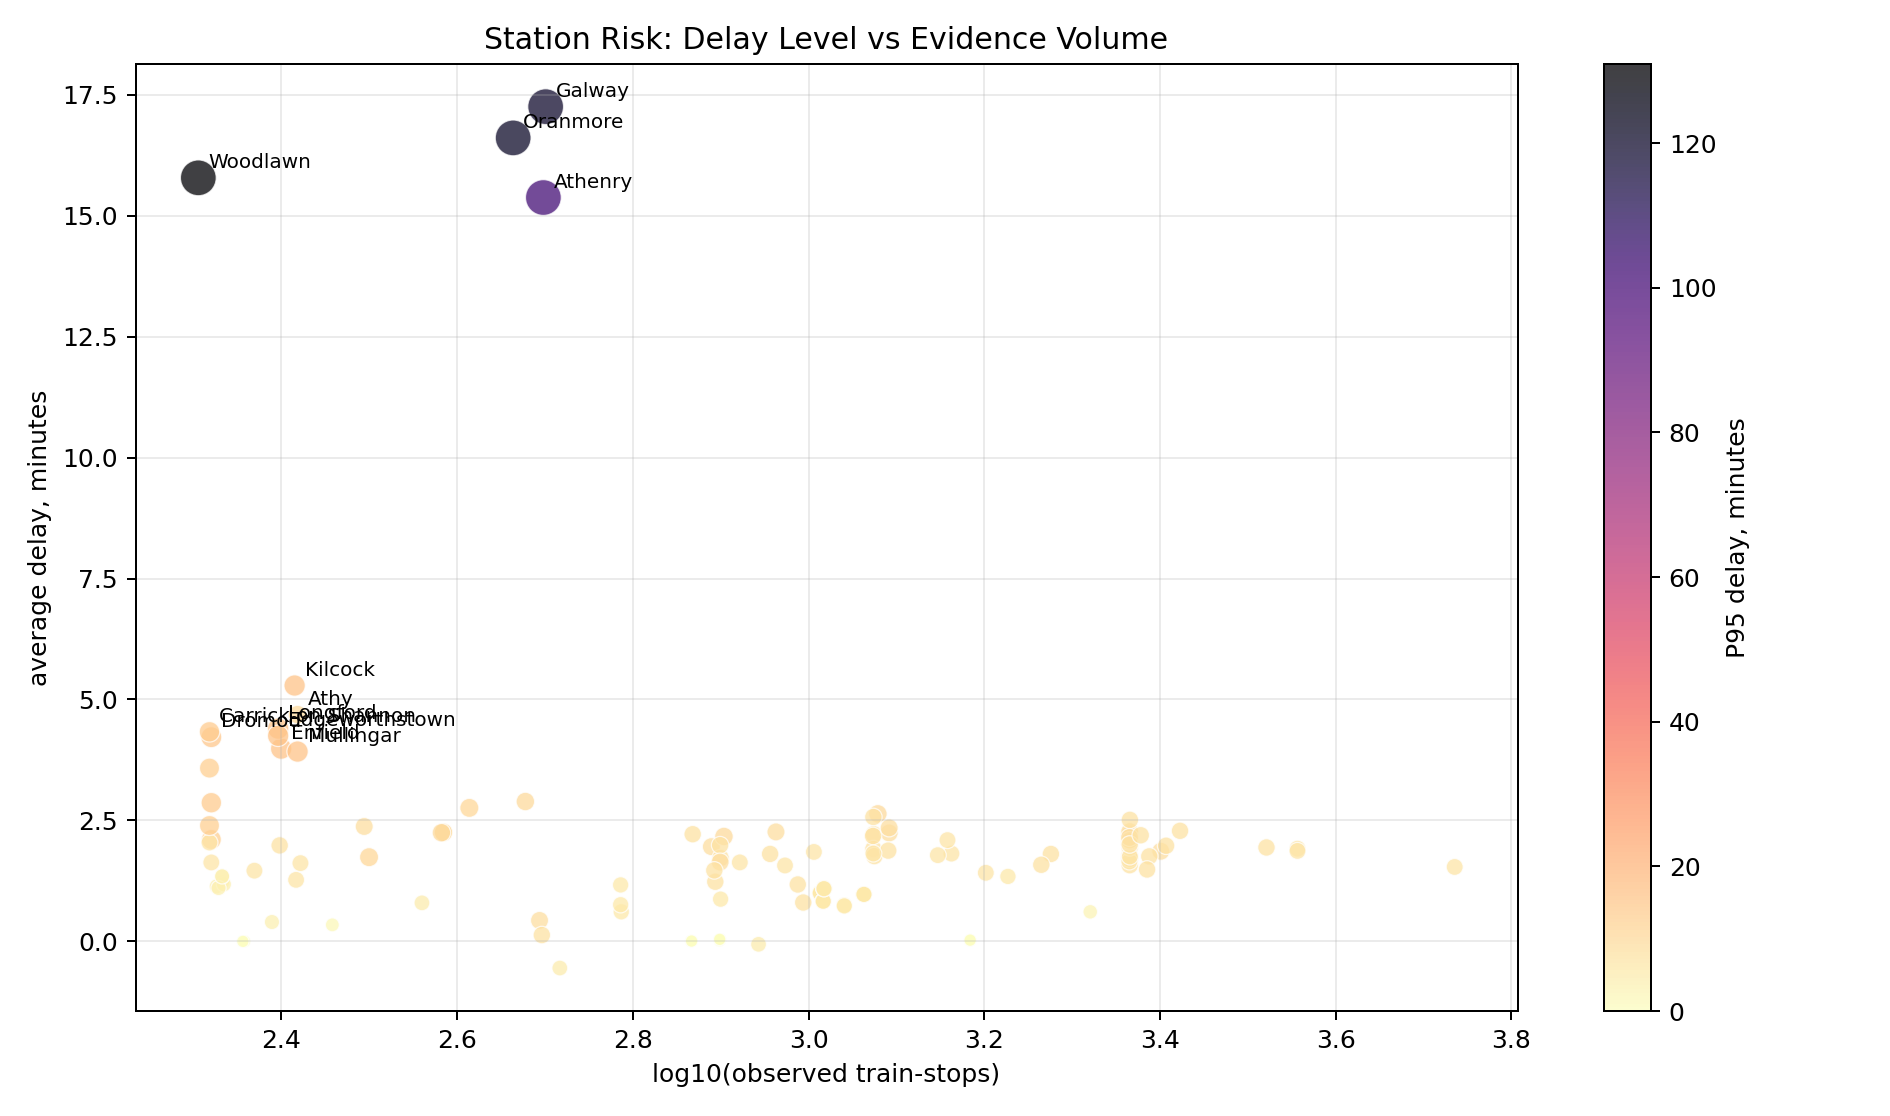
\includegraphics[width=\textwidth]{fig_station_risk.png}
\caption{Each station is a point. The x-axis is evidence volume, the y-axis is average delay, and colour/size encode the upper tail. Galway, Oranmore, and Athenry are high-delay stations with enough evidence to take seriously.}
\end{figure}

\begin{figure}[H]
\centering
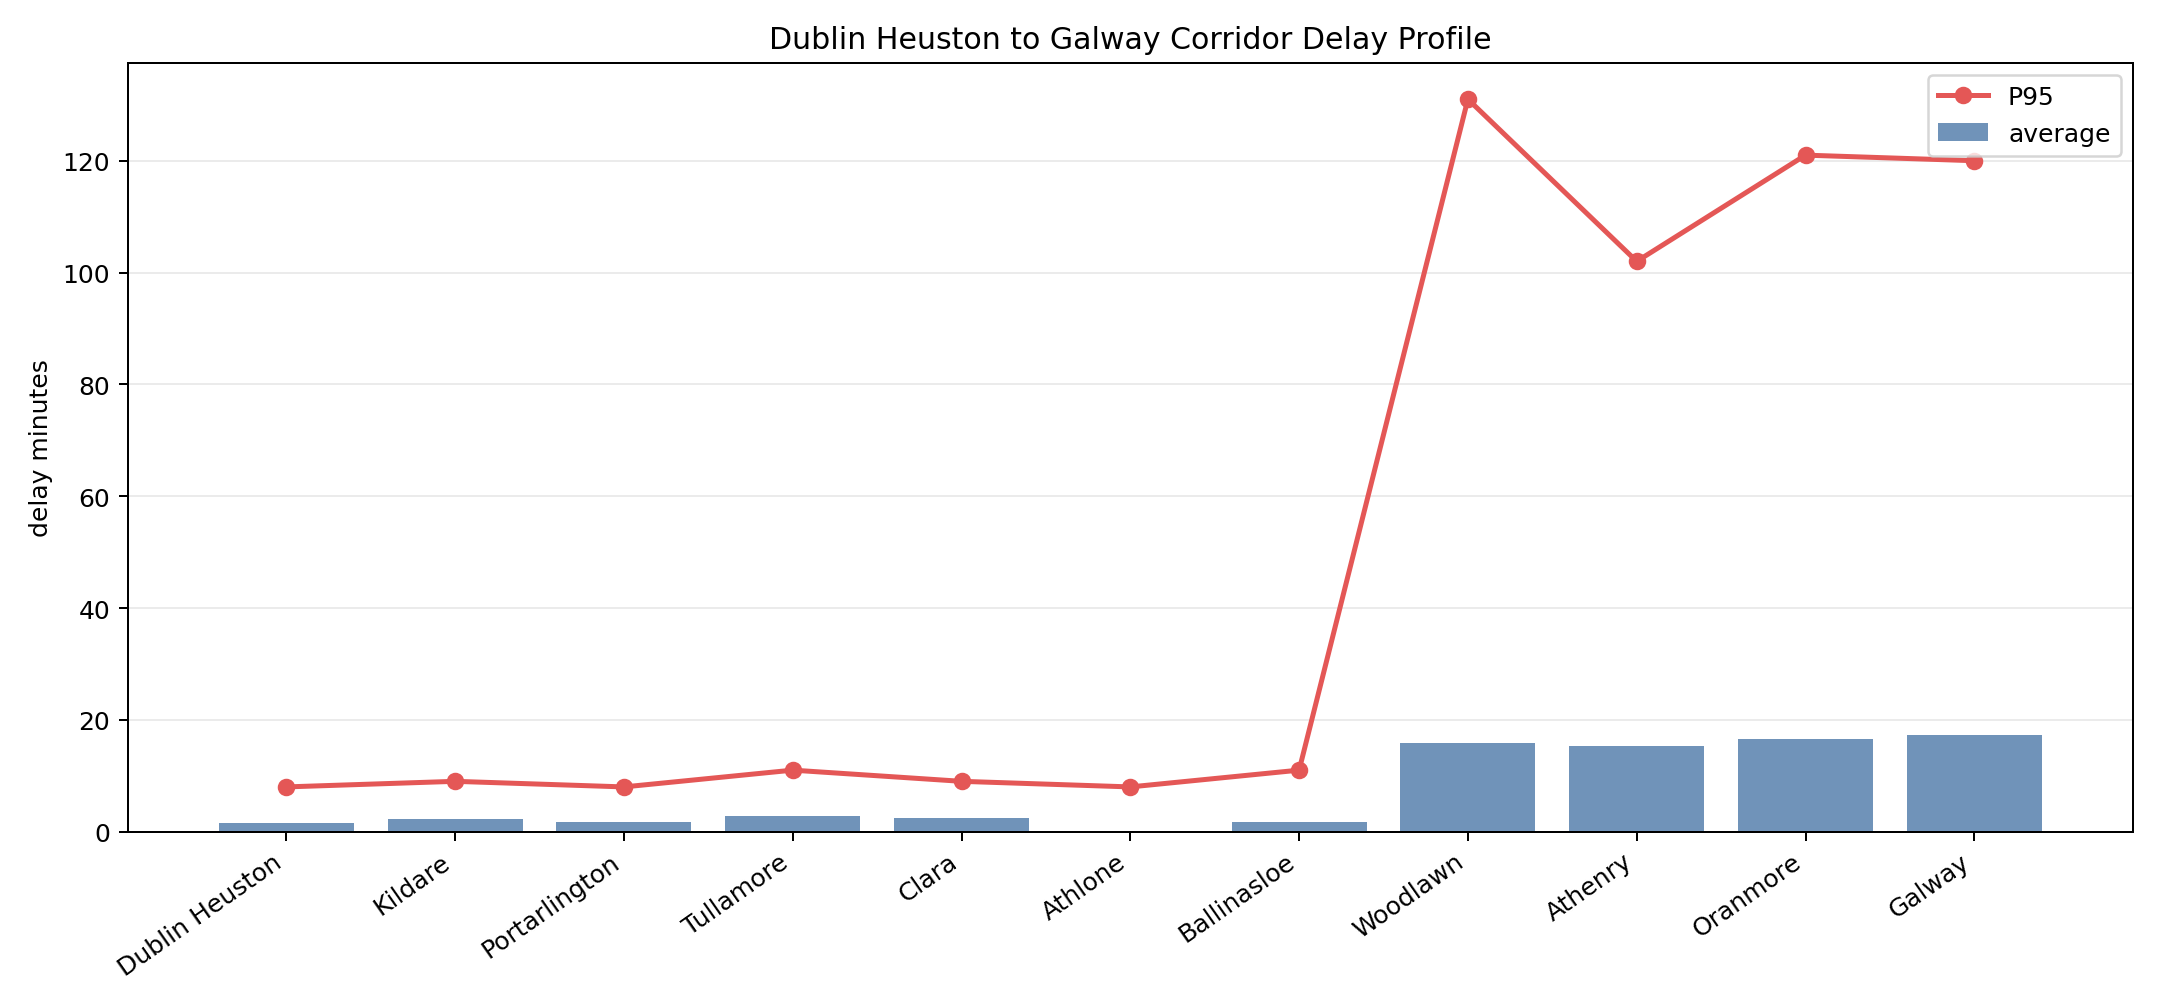
\includegraphics[width=\textwidth]{fig_galway_corridor.png}
\caption{Delay profile along the Dublin Heuston to Galway corridor. The rise around Athenry--Oranmore--Galway is the cleanest operational story in the current sample.}
\end{figure}

\begin{table}[H]
\centering
\small
\begin{tabular}{lrrrr}
\toprule
route & trains & avg & p95 & within5 \\
\midrule
Dublin Heuston to Galway & 144 & 18.61 & 118.00 & 70.23 \\
Dublin Heuston to Westport & 48 & 5.99 & 23.00 & 70.79 \\
Dublin Connolly to Rosslare Europort & 53 & 3.86 & 13.00 & 77.39 \\
Dublin Connolly to Sligo & 109 & 3.60 & 15.00 & 77.42 \\
Sligo to Dublin Connolly & 107 & 3.45 & 13.00 & 82.52 \\
Dublin Heuston to Cork & 198 & 3.41 & 12.00 & 80.02 \\
Dublin Connolly to Belfast & 195 & 3.40 & 12.00 & 78.05 \\
Dublin Connolly to Hazelhatch & 32 & 2.88 & 8.00 & 82.53 \\
Howth to Greystones & 228 & 2.86 & 10.00 & 85.62 \\
Dublin Heuston to Waterford & 110 & 2.76 & 9.00 & 84.39 \\
\bottomrule
\end{tabular}
\caption{Highest average-delay route pairs with at least 20 train codes and 100 cleaned observations. Values are in minutes except within5, which is percent.}
\end{table}

\begin{figure}[H]
\centering
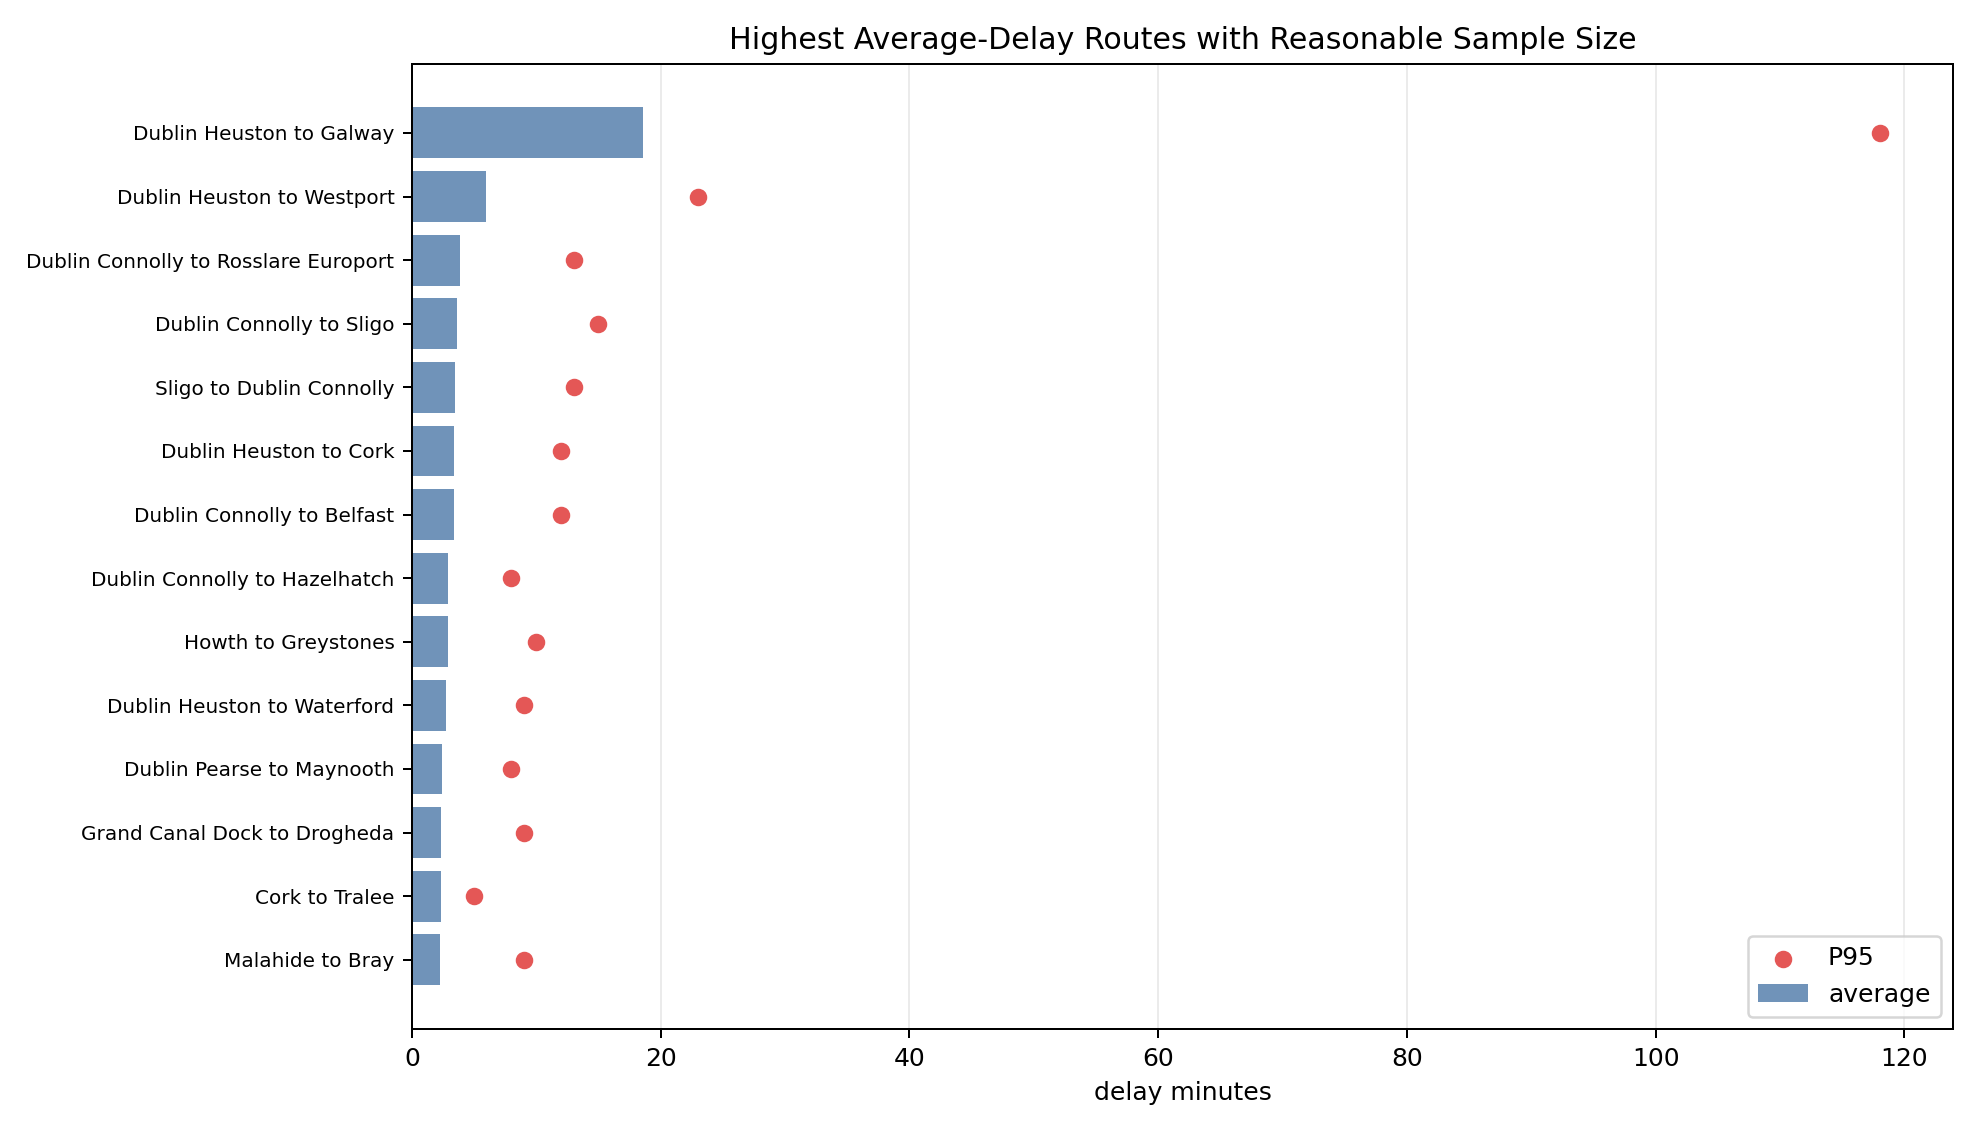
\includegraphics[width=\textwidth]{fig_route_ranking.png}
\caption{Route-level average delay and P95 delay. This avoids over-reading single tiny samples by requiring both route volume and distinct train counts.}
\end{figure}

\section{Chokepoint Analysis}

The station ranking says where trains are late; the chokepoint calculation asks a sharper question: where does delay get added between two consecutive observed stops? For each train/date/route, stops are ordered by scheduled time and the segment delay gain is
\[
\Delta_e = \text{late}(\text{next station}) - \text{late}(\text{previous station}).
\]
Positive $\Delta_e$ means the train became later across that observed segment. To avoid a single bad stale record dominating the result, this transition analysis uses the stricter range
\[
 -30 \leq \text{late minutes} \leq 60.
\]

The current strongest recurring delay-gain segment is \textbf{Attymon to Athenry}: average gain 22.51 minutes, median gain 7 minutes, and P90 gain 61 minutes. On the Dublin Heuston--Galway route specifically, the strongest segment is \textbf{Attymon to Athenry}, with average gain 19.59 minutes and P90 gain 62 minutes.

\begin{table}[H]
\centering
\small
\begin{tabular}{lrrrrr}
\toprule
segment & obs & avg\_gain & med\_gain & p90\_gain & gain\_gt2 \\
\midrule
Attymon to Athenry & 59 & 22.51 & 7.00 & 61.00 & 79.66 \\
Woodlawn to Athenry & 76 & 15.53 & 3.00 & 39.00 & 55.26 \\
Carlow to Athy & 135 & 4.59 & 4.00 & 10.00 & 77.04 \\
Dublin Heuston to Thurles & 41 & 6.78 & 4.00 & 12.00 & 56.10 \\
Dublin Heuston to Newbridge & 102 & 4.21 & 4.00 & 6.00 & 72.55 \\
Monasterevin to Kildare & 267 & 3.24 & 3.00 & 5.00 & 77.90 \\
Drogheda to Dublin Connolly & 193 & 3.50 & 3.00 & 7.00 & 53.37 \\
Dublin Heuston to Ballybrophy & 35 & 3.94 & 3.00 & 8.00 & 60.00 \\
Dundalk to Drogheda & 231 & 3.27 & 3.00 & 8.00 & 54.98 \\
Dublin Connolly to Drogheda & 190 & 3.21 & 2.00 & 9.00 & 45.79 \\
\bottomrule
\end{tabular}
\caption{Top delay-gain chokepoint candidates. \texttt{avg\_gain}, \texttt{med\_gain}, and \texttt{p90\_gain} are minutes added between consecutive observed stops; \texttt{gain\_gt2} is the percent of observations adding more than two minutes.}
\end{table}

\begin{figure}[H]
\centering
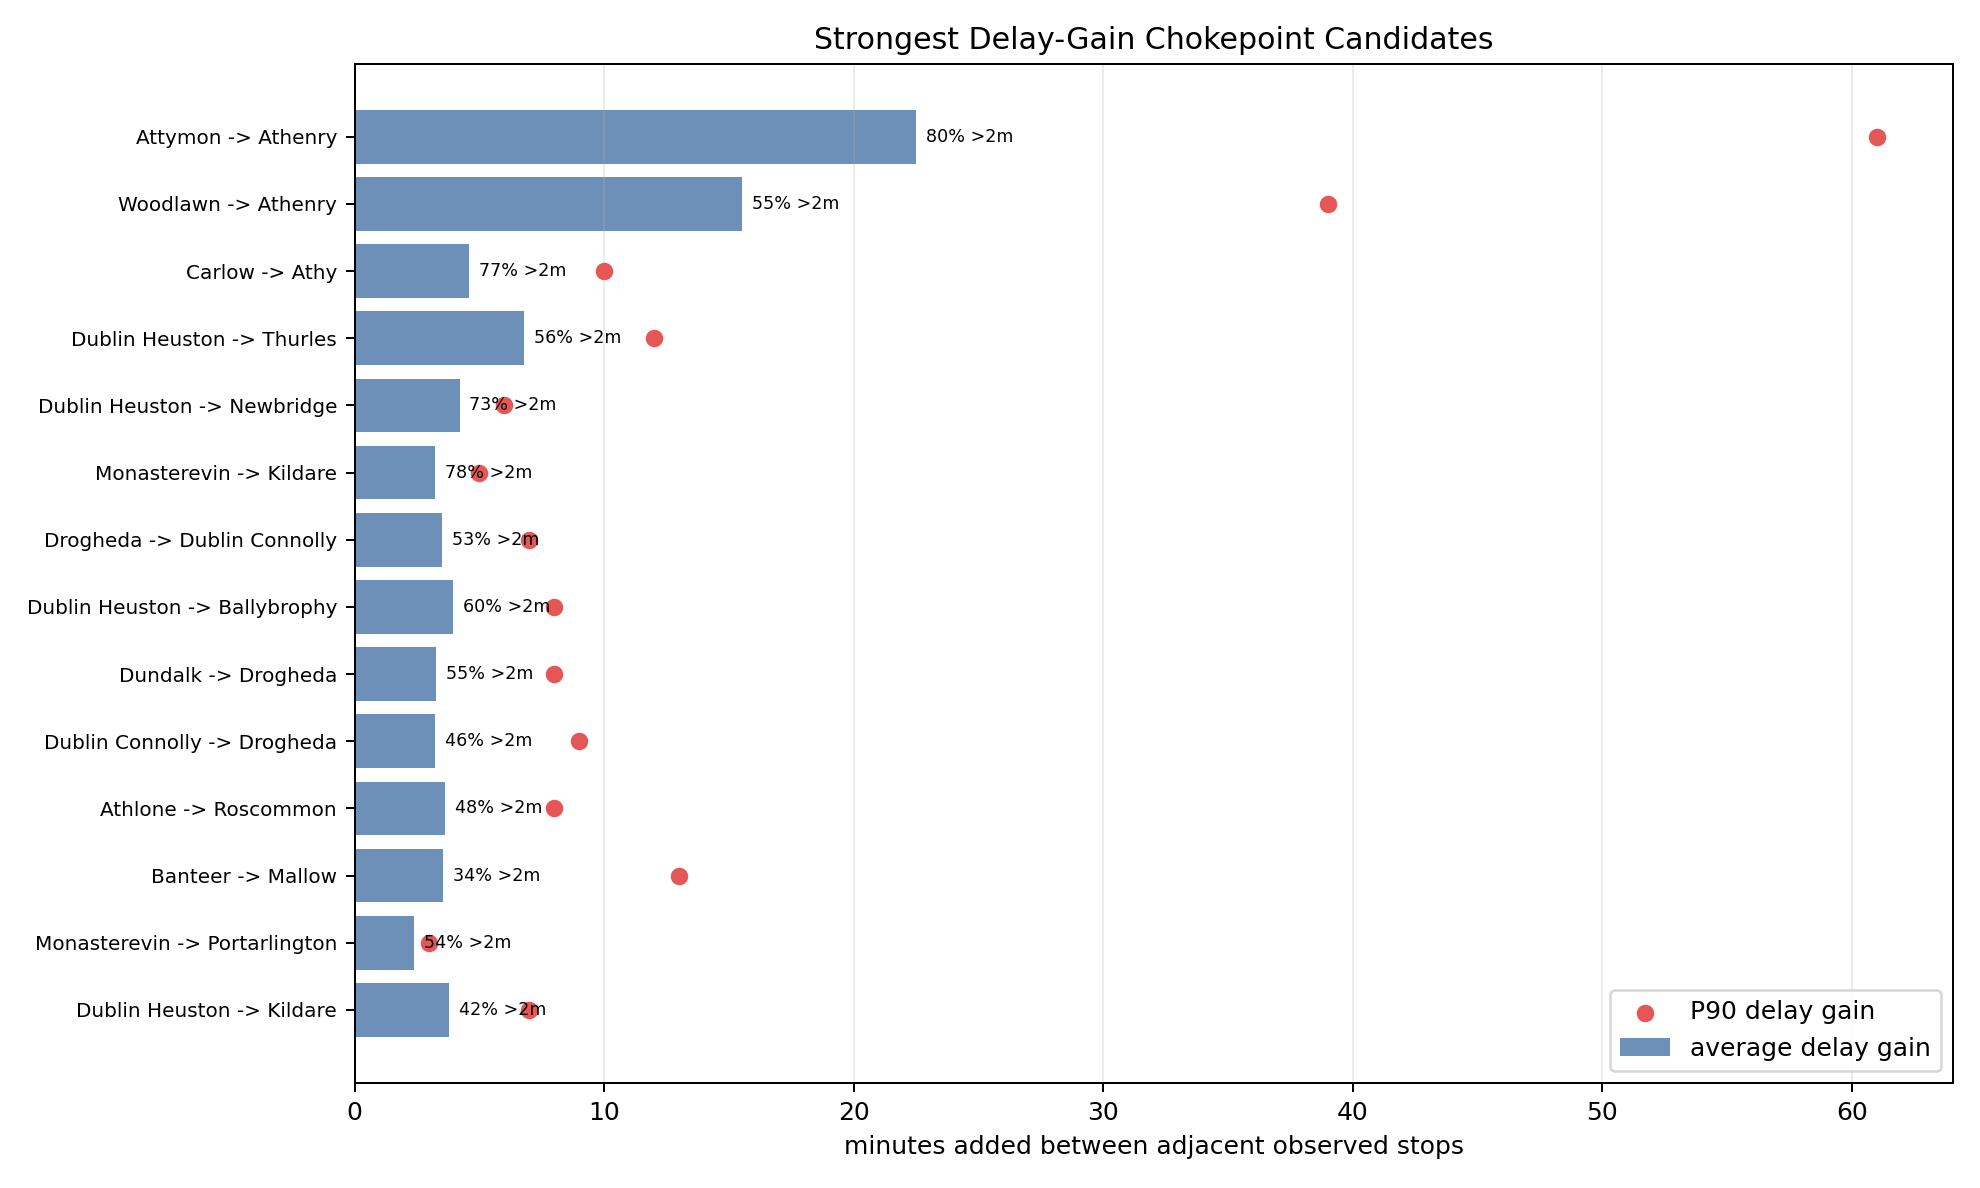
\includegraphics[width=\textwidth]{fig_transition_chokepoints.png}
\caption{Strongest adjacent-stop delay-gain segments. This is the most direct ``where is the chokepoint?'' chart: it measures where lateness increases, not merely where lateness is observed.}
\end{figure}

\begin{figure}[H]
\centering
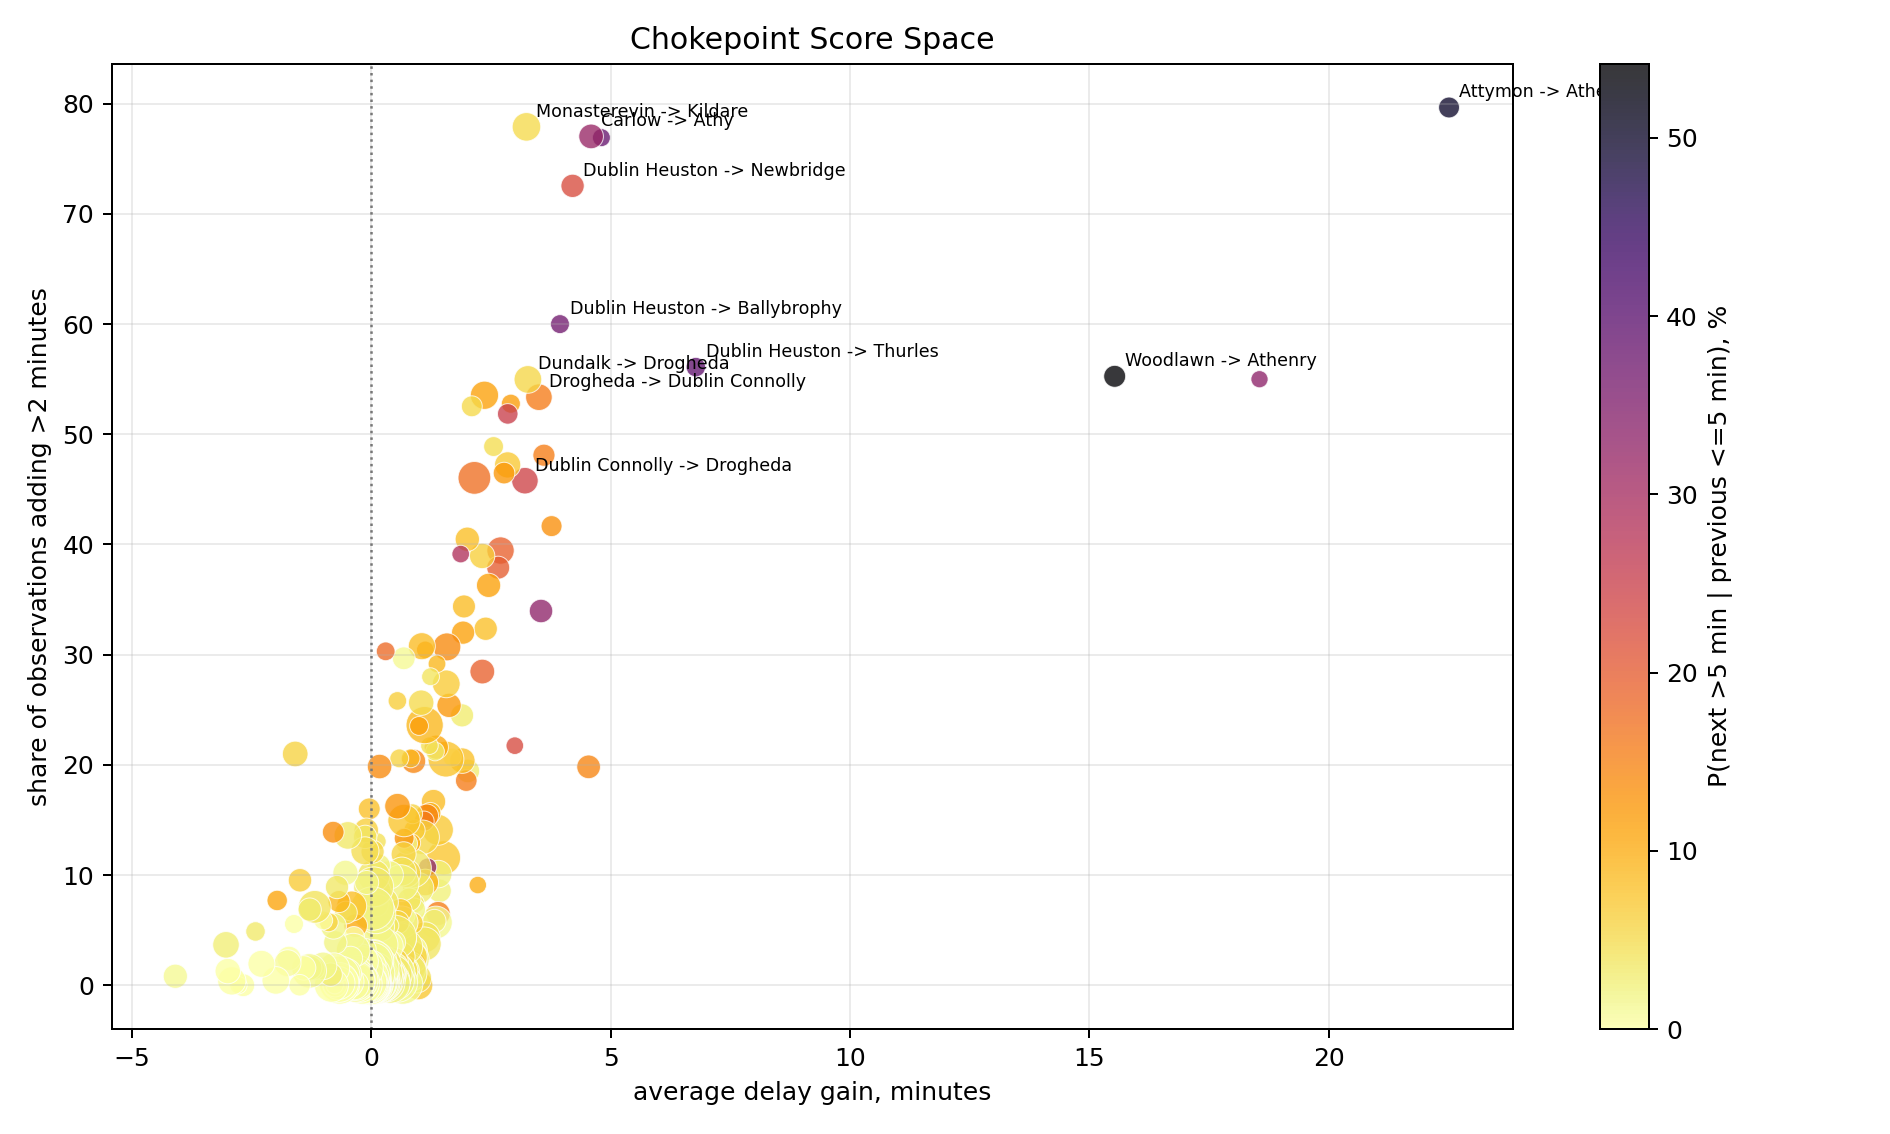
\includegraphics[width=\textwidth]{fig_chokepoint_score.png}
\caption{Chokepoint score space. The best candidates sit high and to the right: many observations, positive average delay gain, frequent gains over two minutes, and high chance of turning an OK train into a late one.}
\end{figure}

\begin{figure}[H]
\centering
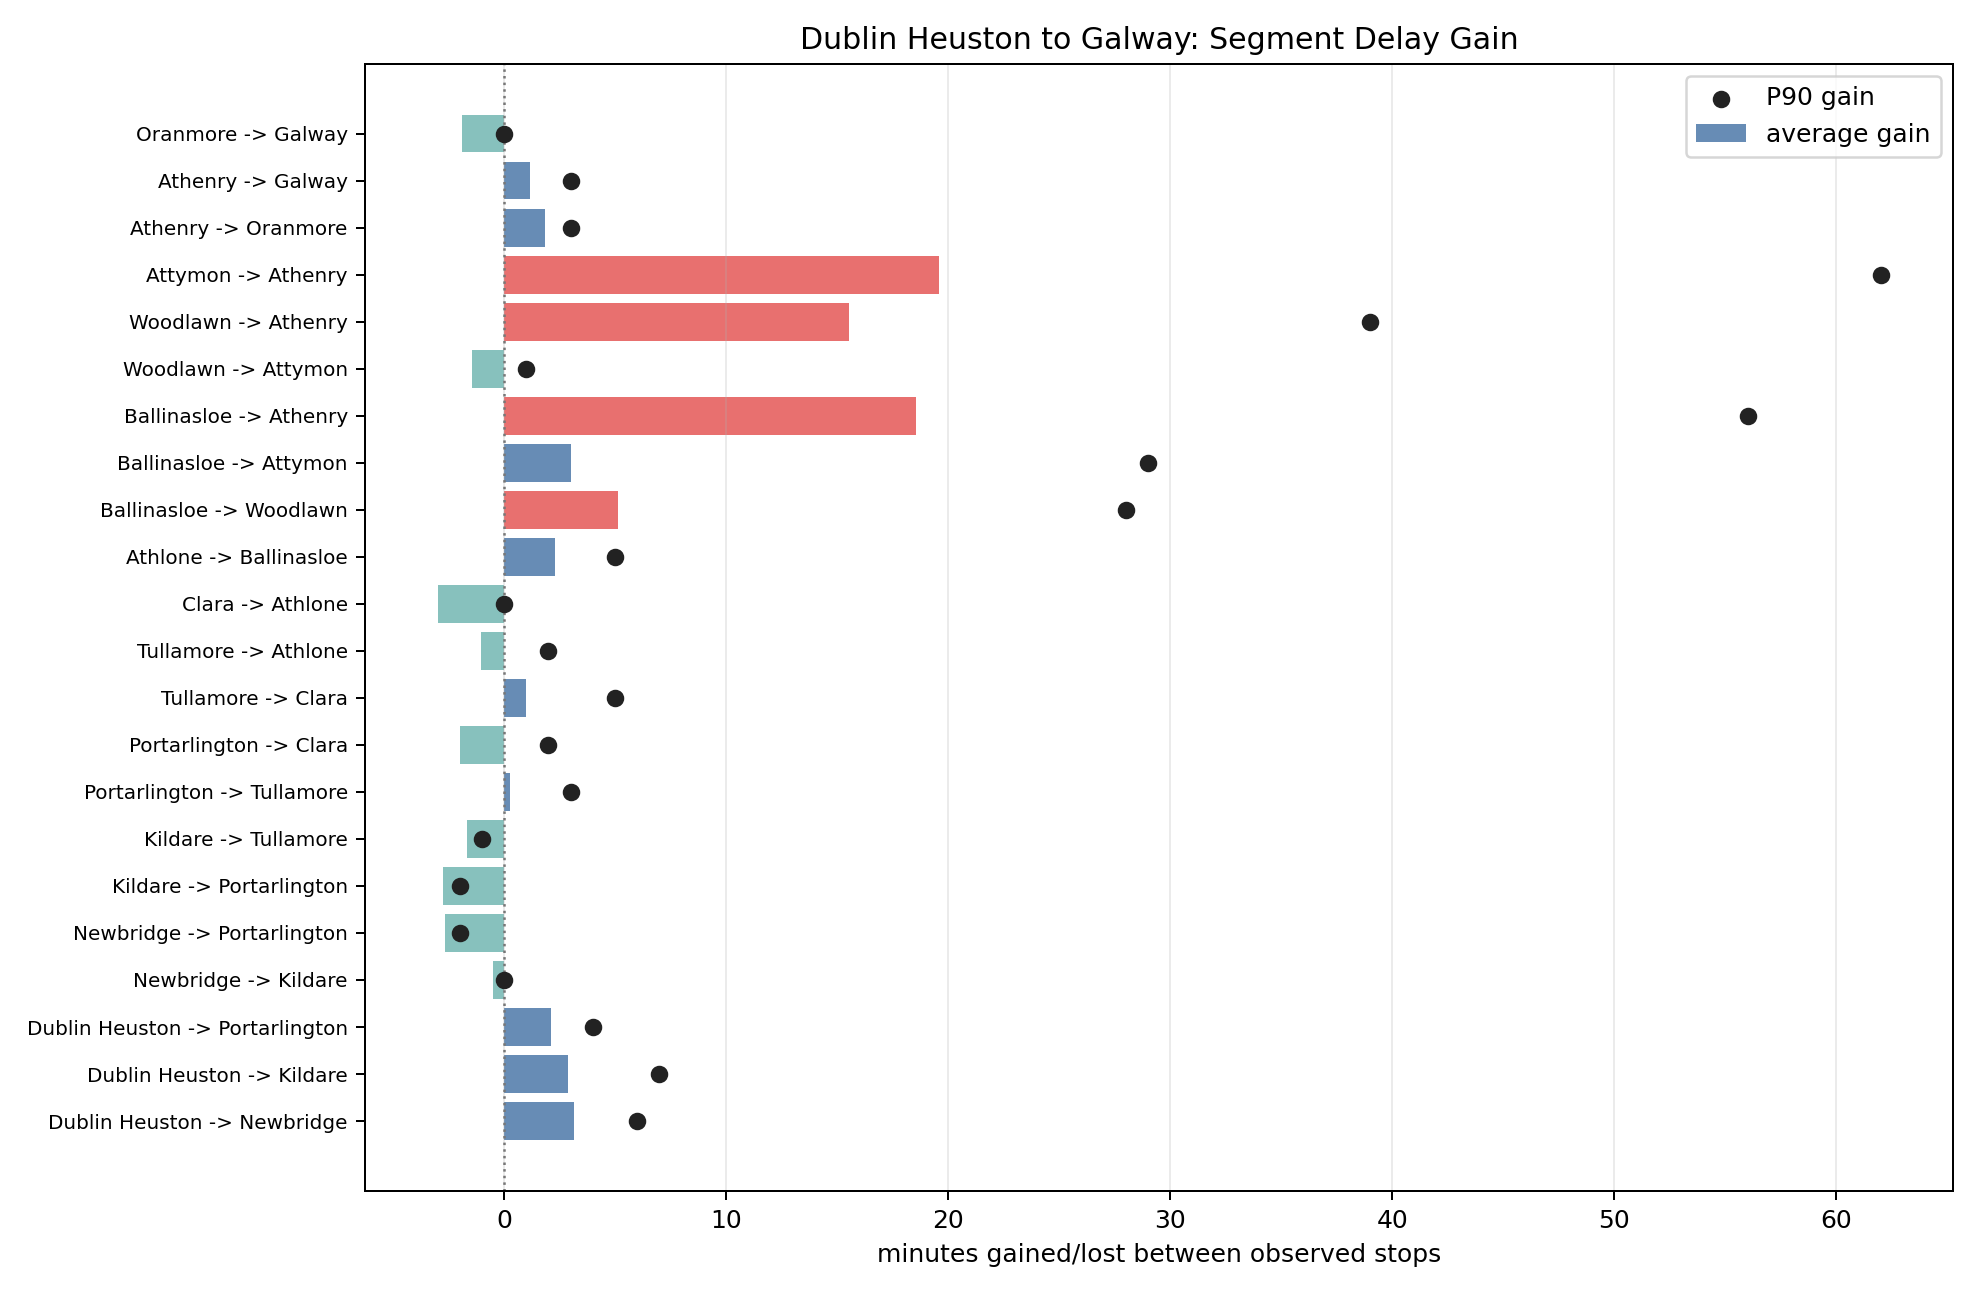
\includegraphics[width=\textwidth]{fig_galway_transition_waterfall.png}
\caption{Dublin Heuston to Galway segment delay gains. The Athenry approach is where the current sample shows the largest recurring delay accumulation; Oranmore and Galway then inherit that lateness.}
\end{figure}

\begin{figure}[H]
\centering
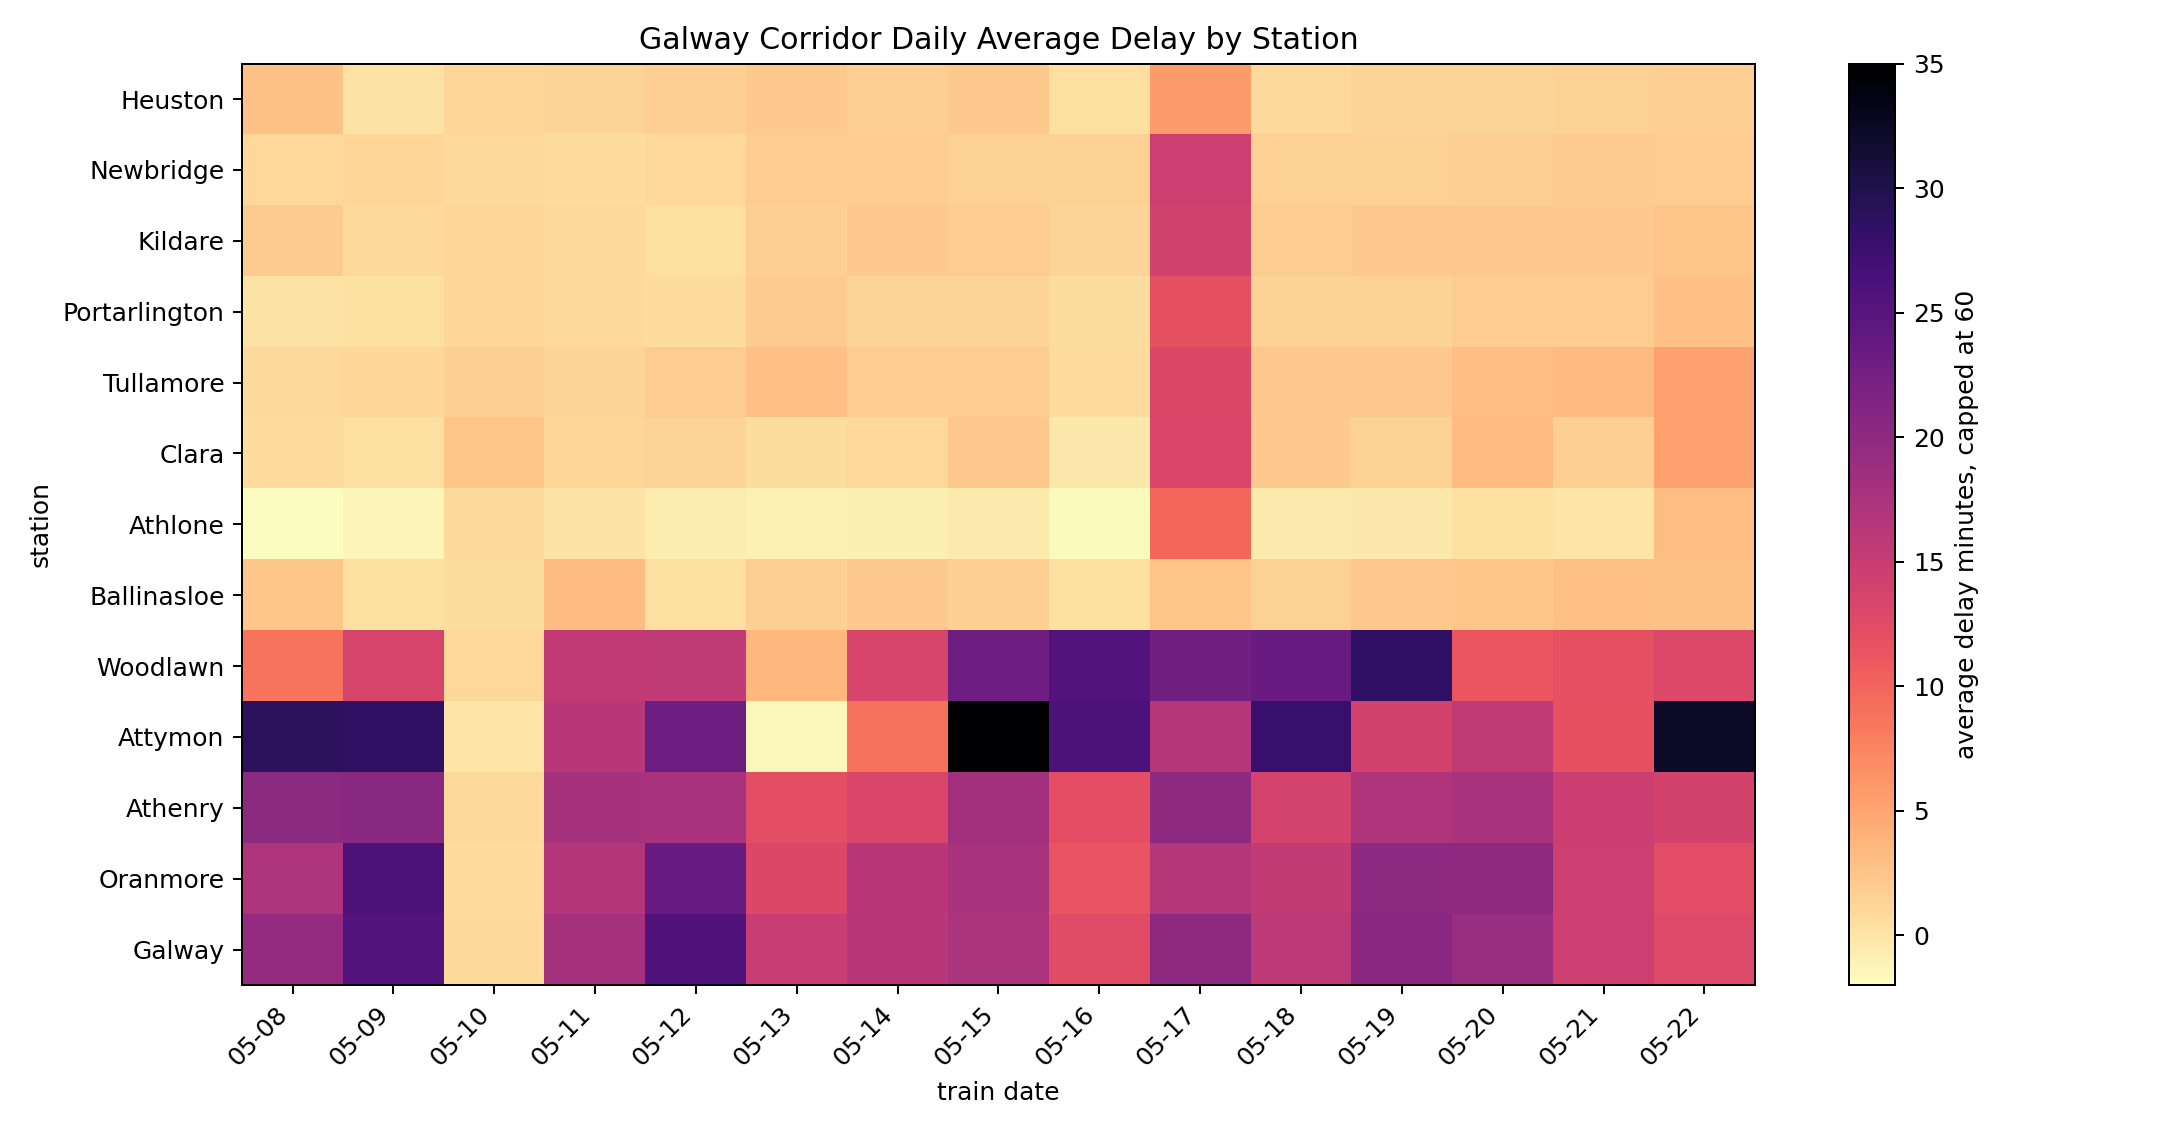
\includegraphics[width=\textwidth]{fig_galway_heatmap.png}
\caption{Daily average delay across the Galway corridor. This separates persistent corridor structure from single-day incidents.}
\end{figure}

\section{Graph View}

For the physical network graph, stations are vertices and rail adjacencies are edges. With weighted adjacency matrix $A$, degree matrix $D$, and Laplacian
\[
L = D - A,
\]
the number of connected components is the nullity of $L$, and the second-smallest eigenvalue $\lambda_2(L)$ measures algebraic connectivity inside a connected component.

The graph model used here has 154 stations in its largest component, 12 physical components, 210 edges, cycle rank 55, and largest-component $\lambda_2 = 0.0013$. The graph is useful, but not perfect: some edges are stitched from geometry fallbacks and some service evidence is missing. Treat the graph math as structure, not gospel.

\begin{figure}[H]
\centering
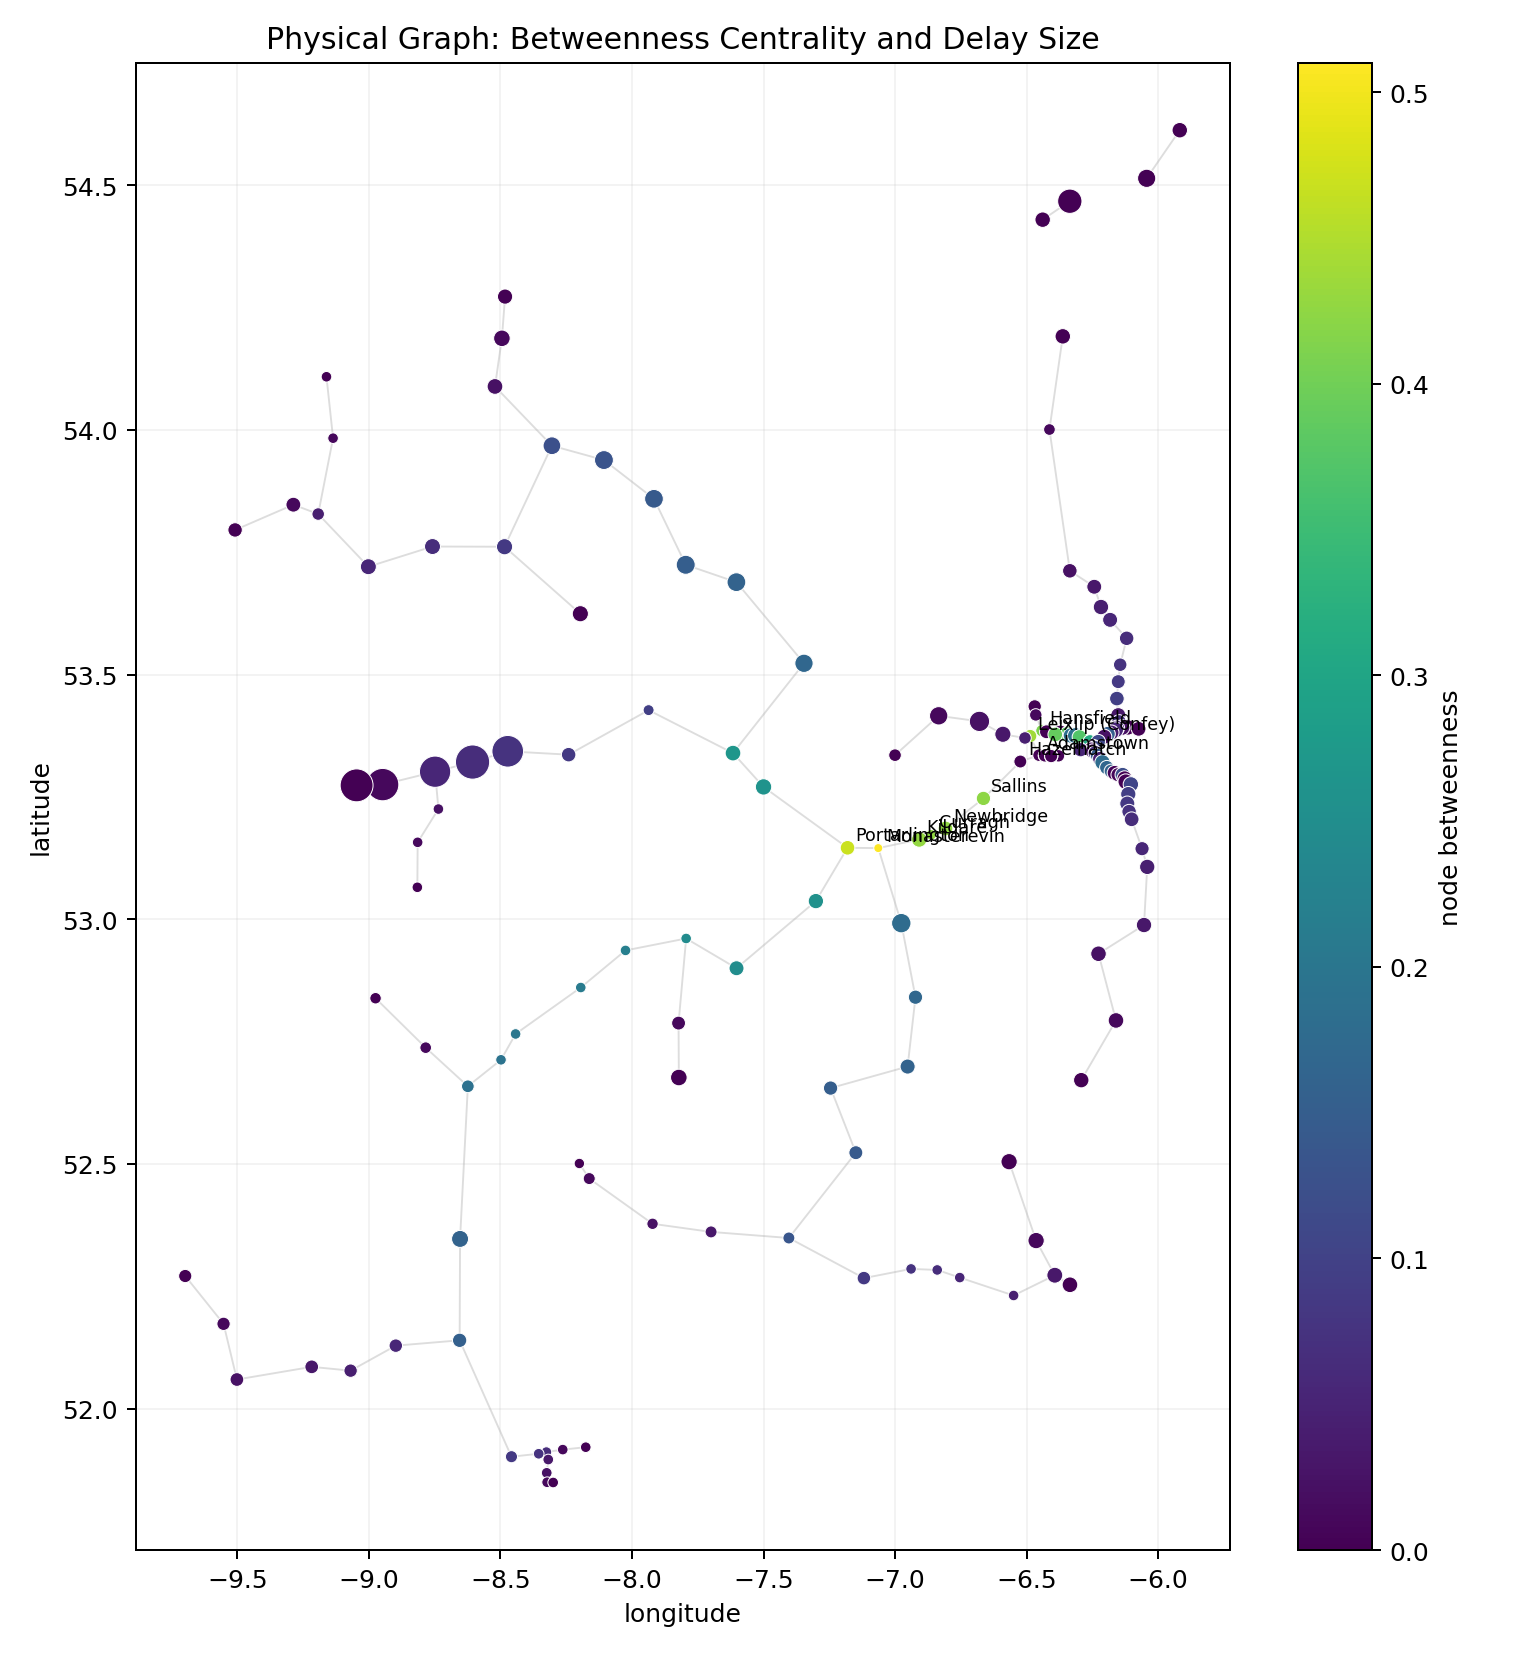
\includegraphics[width=0.9\textwidth]{fig_graph_centrality.png}
\caption{Physical rail graph. Colour is node betweenness centrality: how often a station lies on shortest paths. Point size increases with observed average delay. This separates structural importance from operational pain.}
\end{figure}

\begin{figure}[H]
\centering
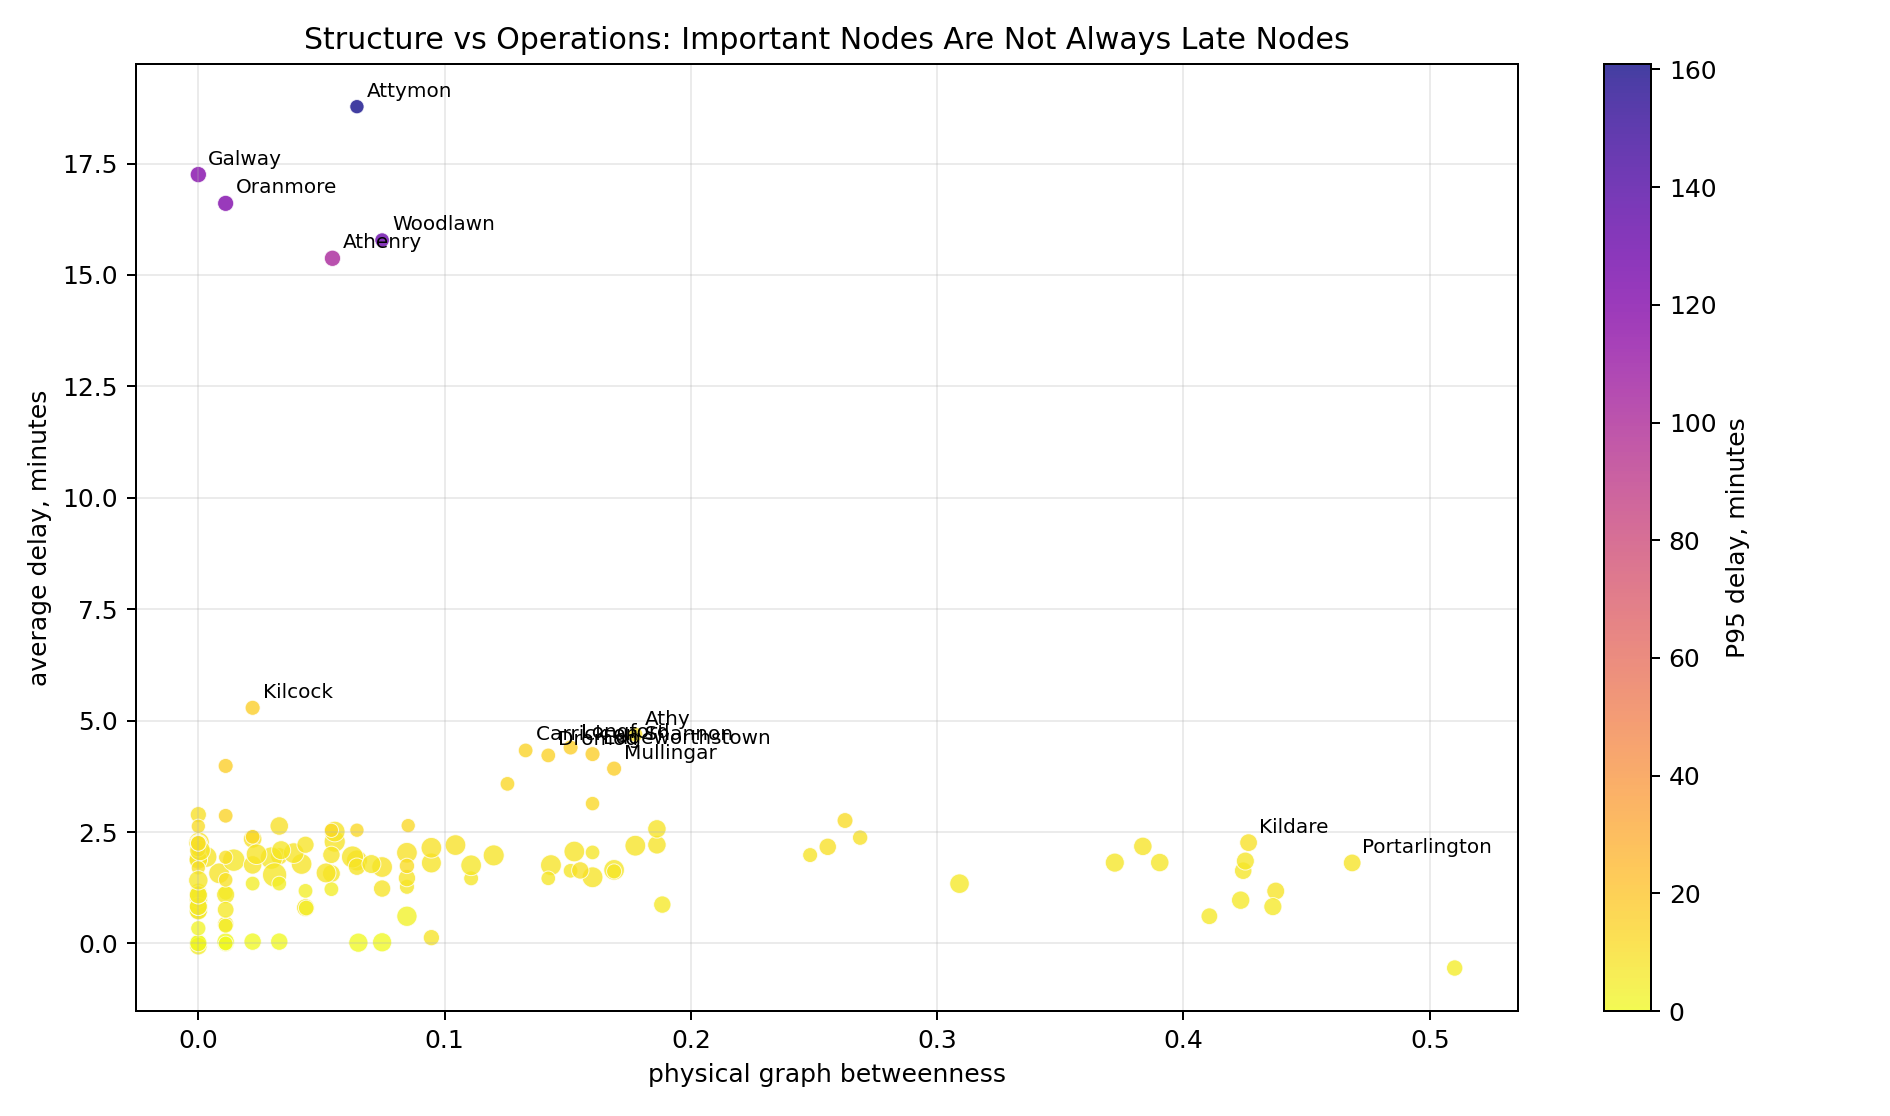
\includegraphics[width=\textwidth]{fig_centrality_delay.png}
\caption{Betweenness centrality versus average delay. Dublin nodes are structurally central; Galway-side nodes are operationally late. Those are different mathematical statements, and both are useful.}
\end{figure}

\begin{figure}[H]
\centering
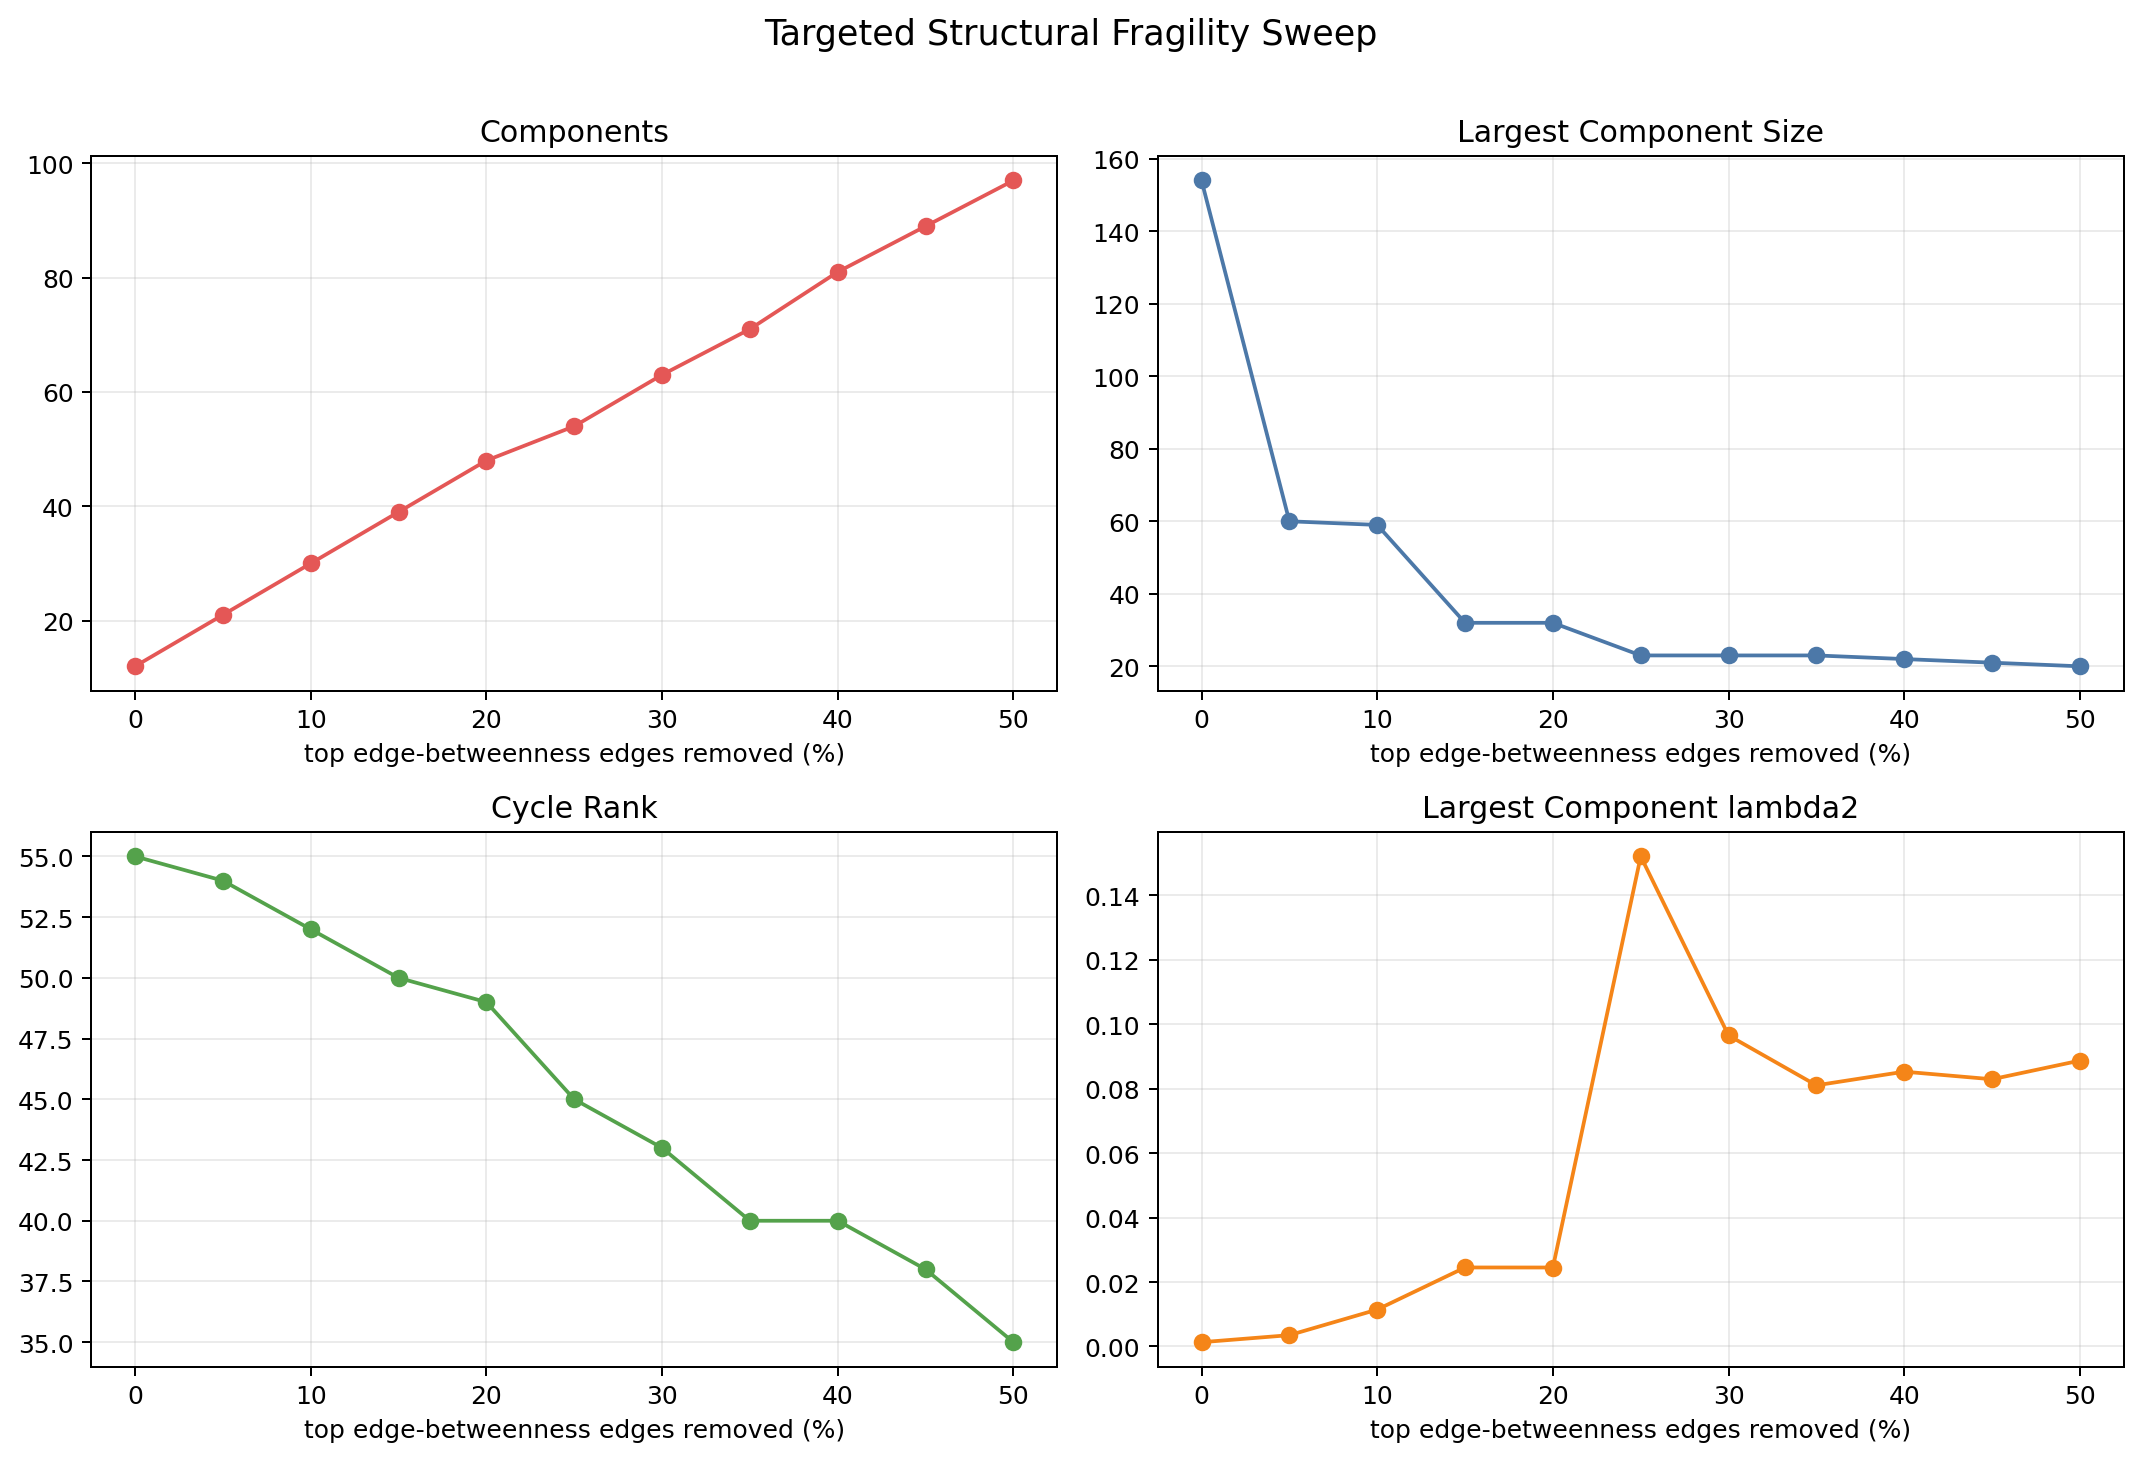
\includegraphics[width=\textwidth]{fig_fragility_sweep.png}
\caption{Targeted removal sweep. Edges are ranked by edge betweenness and removed in 5\% steps. Components, largest component size, cycle rank, and $\lambda_2$ show how fragile a corridor-like rail graph is under targeted cuts.}
\end{figure}

\section{HACON Snapshot Check}

HACON gives a separate delay-like signal through \texttt{difference\_seconds}. In the last 14 days, the cleaned HACON sample has 279,929 snapshots, average difference 2.64 minutes, median 1.4 minutes, P95 9.1 minutes, and 15.6\% over 5 minutes.

\begin{figure}[H]
\centering
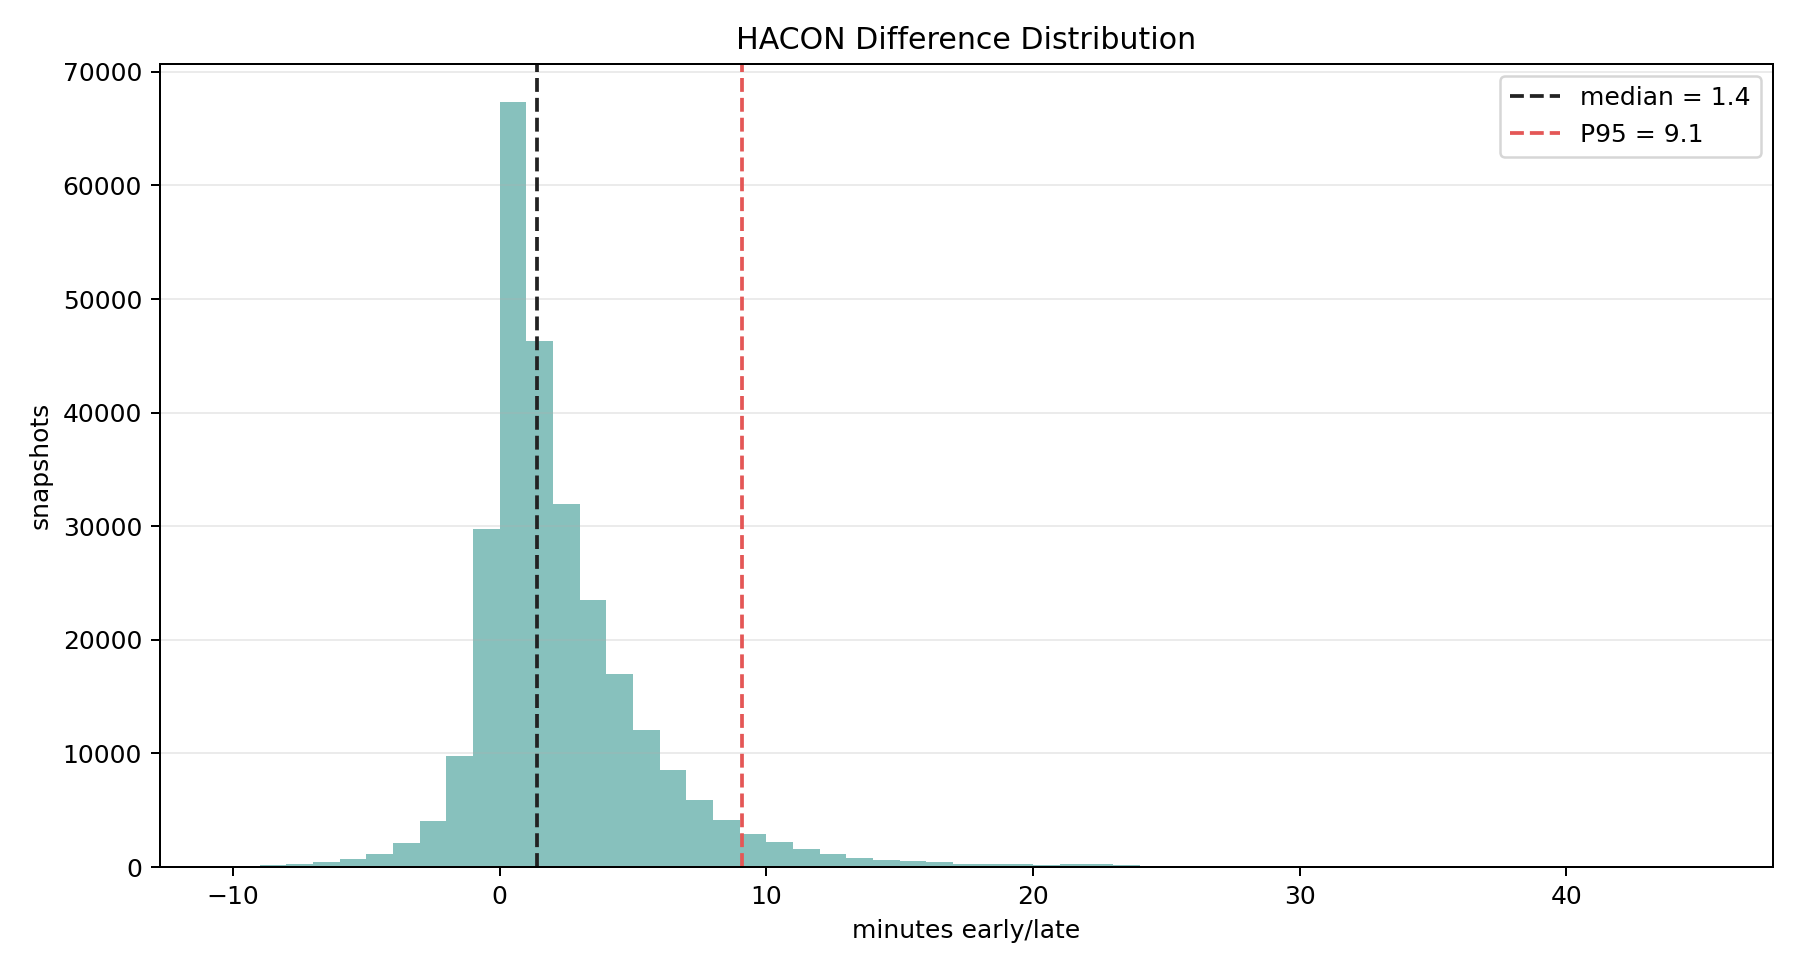
\includegraphics[width=0.9\textwidth]{fig_hacon_distribution.png}
\caption{HACON difference distribution. This is snapshot-based rather than train-stop-based, so it should confirm broad shape rather than replace station-board delay analysis.}
\end{figure}

\section{What This Means}

The archive is now large enough for more than dashboard summaries. The strongest next mathematical directions are:

\begin{itemize}
\item \textbf{Current chokepoint}: in this sample, the clearest measured delay-adding section is the Athenry approach, especially Attymon to Athenry. Operationally, Athenry is where the Galway-line problem becomes visible, while Oranmore/Galway inherit the delay.
\item \textbf{Delay propagation}: estimate $P(D_{v,t+\Delta}>5 \mid D_{u,t}>5)$ along corridors and rank edges by downstream amplification.
\item \textbf{Bayesian station reliability}: shrink low-sample stations toward the network mean so rural/noisy stations do not dominate rankings by accident.
\item \textbf{Robust quantile prediction}: predict P50/P90 delay rather than a single average.
\item \textbf{Spectral fragility}: continue the Laplacian/eigenvalue work, but report it with explicit graph-confidence caveats.
\end{itemize}

\section{Limits}

The data is much better than the old linear algebra project, but the rail graph itself is still imperfect. Station aliases exist, some physical edges have no observed service coverage, and rural/western live-position quality is weaker. The right interpretation is therefore: operational delay findings are strong where sample size is high; graph-theoretic findings are best read as structural hypotheses.

\end{document}
